\documentclass[master=mti,masteroption=ai]{kulemt}
\setup{title={The ISP Course Selection Puzzle},
  author={Herbert Gorissen},
  promotor={Prof. Gerda Janssens},
  assessor={Prof. Danny De Schreye \and Prof. Bettina Berendt},
  assistant={Matthias van der Hallen}}
% De volgende \setup mag verwijderd worden als geen fiche gewenst is.
\setup{filingcard,
  translatedtitle={The ISP Course Selection Puzzle},
  udc=621.3,
  shortabstract={In dit onderzoek worden de mogelijkheden van het IDP systeem getest voor een specifiek probleem namelijk het ISP probleem. Hierbij moet de student een opleiding zien samen te stellen door te kiezen uit de verschillende mogelijke opleidingsonderdelen voor de door hem/haar gekozen opleiding. Het ISP probleem behoort tot de klasse van interactieve configuratieproblemen, hierbij hoort het systeem de gebruiker te ondersteunen terwijl deze een geldige oplossing probeert samen te stellen. IDP als kennisbank systeem laat toe om verschillende vormen van inferentie uit te voeren zonder de kennis over een probleem opnieuw te moeten formuleren. Deze inferentie technieken kunnen de student bijstaan tijdens het samenstellen van diens ISP. De gebruiker kan tijdens deze selectieprocedure foute selecties maken die niet geldig zijn volgens de regels. Conflict explanation is de term die gebruikt wordt voor technieken de verklaringen zoeken voor conflicten. In deze thesis wordt gekeken hoe goed sommige van deze technieken het doen.}
}
\setup{font=lm}

\usepackage[pdfusetitle,colorlinks=false,plainpages=false,hidelinks]{hyperref}
\usepackage{natbib}
\usepackage{ulem}
\usepackage{listings}
\usepackage{graphicx}
\usepackage{amsmath}
\usepackage{amssymb}
\usepackage[linesnumbered,ruled]{algorithm2e}

\bibliographystyle{plainnat}
\setcitestyle{authoryear}

\begin{document}

\begin{preface}
  
\end{preface}

\tableofcontents*

\begin{abstract}
Bij de start van een opleiding aan de K.U. Leuven is iedere toekomstige student verplicht zijn of haar opleiding samen te stellen uit een hele waaier aan opleidingsonderdelen. De selectie van opleidingsonderdelen is echter onderworpen aan een set van regels die allemaal voldaan moeten zijn wil de student een geldig individueel studieprogramma (ISP) bekomen. We kunnen dit scenario onderbrengen in een specifieke verzameling van problemen, namelijk interactieve configuratieproblemen. Een gebruiker, in dit geval de student is verantwoordelijk voor het kiezen van waarden uit het domein voor de verschillende variabelen. Het systeem is tegelijk verantwoordelijk voor de ondersteuning van de gebruiker gedurende dit proces, zodanig dat de selectie uiteindelijk een geldige oplossing vormt volgens de regels van de theorie. 

In dit onderzoek ligt de focus op IDP, een kennisbank systeem ontwikkeld aan de K.U. Leuven dat toelaat domein specifieke kennis uit te drukken d.m.v. FO(\textperiodcentered) in wat de \textit{theorie} van het probleem genoemd wordt. Met deze kennis kan het bijhorende IDP systeem verscheidene vormen van inferentie toepassen op de theorie. Met inferentie wordt bedoeld vragen over het probleem oplossen. Door deze opsplitsing is de vorm van inferentie niet langer gebonden aan het systeem. IDP is in staat om verschillende soorten vragen over het probleem te beantwoorden zonder dat de kennis erover herschreven moet worden.

Sinds het ontstaan van IDP zijn er reeds verschillende onderzoeken gedaan naar de prestaties van IDP op grote problemen \citep{van2016kb} \citep{vlaeminck2009logical}. De resultaten hiervan zijn positief, en onderzoek zal moeten uitwijzen of dit voor het ISP probleem ook het geval is.

Er bestaat al een web applicatie die de studenten bijstaat tijdens het selectieproces van hun opleidingsonderdelen. Door gebruik te maken van de verschillende vormen van inferentie uit het IDP systeem, ben ik ervan overtuigd een applicatie te kunnen ontwikkelen die betere ondersteuning kan bieden en meer mogelijkheden heeft. 

Naast dit alles heeft deze thesis nog een andere grote doelstelling. Sinds een gebruiker verantwoordelijk is voor de selectie van waarden uit het domein, is het mogelijk dat bepaalde combinaties van keuzes nooit een geldige oplossing kunnen zijn volgens de regels. Conflict Explanation is een sub-domein binnen interactieve configuratie waar de focus ligt op het proberen verklaring van deze ongeldige selecties oftewel conflicten. En het is mijn doel om de mogelijkheden van hieromtrent IDP te testen en daarnaast op zoek te gaan naar andere methoden die aan IDP kunnen bijdragen.
\end{abstract}

% Een lijst van figuren en tabellen is optioneel
%\listoffigures
%\listoftables
% Bij een beperkt aantal figuren en tabellen gebruik je liever het volgende:
%\listoffiguresandtables
% De lijst van symbolen is eveneens optioneel.
% Deze lijst moet wel manueel aangemaakt worden, bv. als volgt:
%\chapter{Lijst van afkortingen en symbolen}
%\section*{Afkortingen}
%\begin{flushleft}
%  \renewcommand{\arraystretch}{1.1}
%  \begin{tabularx}{\textwidth}{@{}p{12mm}X@{}}
%    IDP  & Imperative/Declarative Programming \\
%    ISP  & Individueel Studieprogramma \\
%    ASP  & Answer Set Programming \\
%    CSP  & Constraint Satisfaction Problem \\
%    IC   & Interactief Configuratieprobleem \\
%  \end{tabularx}
%\end{flushleft}
%\section*{Symbolen}
%\begin{flushleft}
%  \renewcommand{\arraystretch}{1.1}
%  \begin{tabularx}{\textwidth}{@{}p{12mm}X@{}}
%    $c$   & Lichtsnelheid \\
%    $E$   & Energie \\
%    $m$   & Massa \\
%    $\pi$ & Het getal pi \\
%  \end{tabularx}
%\end{flushleft}

% Nu begint de eigenlijke tekst
\mainmatter

\chapter{Inleiding}
\label{inleiding}

\subsection{Constraint Satisfaction Problems}
CSP's zijn problemen waar voor een reeks variabelen een geldige waarde uit het domein dient toegekend te worden. De toekenning echter is gebonden aan een set van regels waaraan de variabelen moeten voldoen. Formeel defini\"{e}ren we een CSP als een triple $\langle \mathcal{X},\mathcal{D},\mathcal{C} \rangle$, met $\mathcal{X}$ de verzameling van variabelen, $\mathcal{D}$ de domeinwaarden voor deze variabelen en $\mathcal{C}$ de constraints over de variabelen. Typisch worden dit soort problemen opgelost d.m.v. zoeken door alle mogelijk combinaties, deze recursieve methode gaat voor elke nieuwe toekenning na of de constraints voor de parti\"{e}le toekenning consistent zijn. Zo ja, dan volgt er een nieuwe recursieve oproep, anders gaat het algoritme backtracken. Het oplossen van CSP's met een eindig domein behoort tot de klasse van NP-complete problemen en de berekeningen zijn vaak van hoge complexiteit met betrekking tot de grootte van het domein. Om het zoekproces proberen te versnellen bestaan er variaties op backtracking zoals backmarking en backjumping. De eerste zorgt voor een effici\"{e}ntere manier om consistentie na te gaan en backjumping is een betere manier van backtracking waarbij men over meerdere waarden tegelijk kan backtracken. Deze technieken versnellen het zoekproces in dat ze onnodige stappen detecteren en overslaan. Anderzijds bestaan er propagatie technieken die lokale consistentie garanderen met technieken zoals arc consistency, hyper-arc consistency en path-consistency die de domeinen van de variabelen proberen te verkleinen alvorens het zoekproces gestart wordt. Naast dit soort technieken wordt er ook vaak gebruik gemaakt van zoekalgoritmen die gebruik maken van heuristieken om de grote zoekruimte van een probleem te proberen verkleinen en zo sneller tot een oplossing te komen. Wanneer voor elke variabele $\mathcal{X}_{i}$ een waarde uit diens domein $\mathcal{D}_{i}$ is toegekend door het zoekproces en voor deze combinatie van toekenning geldt dat elke constraint $\mathcal{C}_{j} \in \mathcal{C}$ consistent is, dan wordt er gesproken van een oplossing. 

\subsection{Interactive Configuration Problems}
In deze thesis ligt de focus op een specifieke groep van problemen binnen het domein van CSP's genaamd Interactieve Configuratieproblemen (IC). Constraint Satisfaction Problems zijn problemen waar een toekenning van domeinwaarden voor de variabelen dient gevonden te worden waarvoor geldt dat aan alle constraints voldaan is. IC problemen hebben hetzelfde doel, maar bij CSP's wordt er naar een toekenning gezocht d.m.v. recursieve zoektechnieken terwijl het in het geval van IC problemen een gebruiker is die handmatig stap per stap een geldige toekenning gaat proberen samenstellen. Om de gebruiker hierin bij te staan is er nood aan software die de gebruiker zo goed mogelijk bijstaat gedurende dit hele proces. Uit ervaring is gebleken dat het schrijven van software voor dit soort problemen geen gemakkelijke opgave is. Zo is aangetoond dat een imperatieve aanpak voor het beschrijven van de regels van een probleem vaak moeilijk is \citep{gelle1996interactive}. Reden hiervoor is dat de regels over de betreffende domeinkennis vaak verspreid zit in de software in codesnippets. Daarbij is onderhoud van zulke software een enorm moeilijke opgave waarbij de kleinste wijziging in de constraints kan leiden tot een volledige herwerking van de code. Een alternatief hiervoor is een declaratieve aanpak. In declaratieve toepassingen kunnen de regels van een probleem beschreven worden d.m.v. logische constraints. \cite{gelle1996interactive} laten niet alleen zien dat de declaratieve beschrijving van een probleem overzichtelijker en duidelijker is maar ook dat een wijziging in de constraints gemakkelijk aangepast kan worden. En hoewel er met een imperatieve aanpak meer optimale algoritmen ontwikkeld kunnen worden, is aangetoond dat declaratieve methoden ook goede prestaties kunnen neerzetten. Het werk van\citep{vlaeminck2009logical} legt gelijkaardige argumenten voor. De paper verwijst naar een voorbeeld (Tax on web) waarbij een imperatieve aanpak inderdaad nadelig bleek te zijn. Het werk stelt een declaratieve aanpak voor voor het beschrijven van de regels van een probleem en inferentie om vragen erover op te lossen. Ook zij concluderen dat het een veel effici\"{e}ntere manier is voor het beschrijven van een probleem in een overzichtelijke set van logische regels, en dat een declaratieve aanpak toch (voor het gekozen probleem) een goede reactietijd heeft als het aankomt op de inferentie methoden.

\subsection{Declaratieve Systemen}
Er zijn ondertussen vele declaratieve systemen verschenen (Prolog, Ant, Lisp, ...). Wat opvalt is dat elk systeem vaak gebonden is aan \'{e}\'{e}n enkele specifieke vorm van inferentie. Afhankelijk van de gewenste inferentie zal een probleem dus opnieuw moeten beschreven worden in een ander systeem waarmee deze vorm van inferentie wel mogelijk is, ondanks het feit dat de kennis telkens dezelfde is. 

\paragraph{Het IDP Systeem}
Deze gedachtegang ligt aan de basis van het concept van het Kennisbank paradigma \citep{denecker2008building}. In het KB-paradigma wordt gesteld dat de inferentie los staat van de kennis over een probleem. Deze kennis is niets meer dan een verzameling van informatie, maar op deze informatie kunnen meerdere vormen van inferentie toegepast worden. In dit onderzoek ligt de aandacht op IDP, een KB-systeem ontwikkeld aan de K.U. Leuven en voor het eerst voorgesteld in 2008. Het laat toe om de kennis over een probleem te beschrijven in FO(\textperiodcentered), dit is eerste orde logica maar uitgebreid met aggregaten, type definities en inductieve definities. IDP integreert state-of-the-art technologie\"{e}n uit Answer Set Programming (ASP) en SAT solving voor het oplossen van inferentie taken. De architectuur van IDP bestaat uit twee delen, een grounder en een solver. De taak van de grounder is om de input structuur om te vormen tot een formaat dat de solver begrijpt, dit formaat is een extensie van de conjunctieve normaalvorm (ECNF). De solver van het IDP systeem is de MiniSAT(ID) solver \citep{de2014minisat}.

\paragraph{Andere systemen}
IDP is niet het enige systeem waarmee kennis over een probleem kan uitgedrukt worden en er inferentie op kan toepassen. Gringo Clasp \citep{gebser2007clasp} is een populair systeem gebaseerd op technieken van ASP. Het systeem doet aan conflict-driven ASP solving, en maakt gebruik van heuristieken om zo het zoekproces te versnellen. Een ander bekend ASP systeem is DLV, wat toelaat kennis over een probleem uit te drukken d.m.v. disjunctieve logica. Beide systemen zijn uitstekend voor model expansie en zelfs optimisatie, maar zoals vele andere systemen werken zij niet volgens het KB-paradigma. De kennis over de problemen is nog steeds verbonden aan een specifieke vorm van inferentie(s). 

\paragraph{Vergelijking met andere systemen}
IDP dus is niet het enige systeem dat gebruikt zou kunnen worden om te helpen de vragen in dit onderzoek te beantwoorden. IDP en diens notie van het KB-paradigma maken het echter wel een aantrekkelijke kandidaat. Deze motivatie achter deze keuze is ook te wijten aan de resultaten van enkele gerelateerde studies. 

In \citep{wittocx2008idp} wordt de vergelijking gemaakt tussen IDP en ASP solvers. ASP oftewel Answer Set Programming is een populaire techniek voor het berekening van oplossingen (model expansie) voor een logisch probleem. Verscheidene systemen waaronder het bekende \textit{Clasp} zijn een implementatie van het ASP paradigma. IDP zelf maakt gebruik van een combinatie van technieken uit ASP en SAT. In de paper tonen de auteurs het resultaat van een vergelijkende studie tussen verschillende model expansie systemen op een verzameling van problemen. Merk op dat de focus enkel ligt op model expansie en niet op de andere vormen van inferentie die ook mogelijk zijn met IDP. De resultaten tonen dat IDP naast alle andere solvers ook goede prestaties behaalt. Bovenop deze cijfers wordt ook nog eens benadrukt dat de rijke en elegante taal die IDP gebruikt voor het beschrijven van problemen wellicht het belangrijkste onderdeel is van het systeem. Het gebruik van eerste orde logica uitgebreid met aggregaten, types, inductieve definities, parti\"{e}le functies, rekenkundige bewerkingen enz. maakt het beschrijven van problemen veel makkelijker wat uiteindelijk de taak van het modelleren h\'{e}\'{e}l wat simpeler maakt.

\citep{de2014minisat} is een vergelijkende studie tussen MiniSAT(ID) solver uit IDP en Gringo-Clasp. De laatste was de winnaar van de ASP wedstrijd in 2013 voor de categorie Model-and-Solve waar IDP als vierde eindigde. Voor sommige van de problemen werd IDP echter gediskwalificeerd door problemen met het modelleren. Daarom hebben de auteurs IDP opnieuw getest tegen de problemen van de wedstrijd en de resultaten vergeleken met die van Gringo-Clasp. De uitkomst tonen dat Gringo-Clasp meer instanties van de problemen heeft kunnen oplossen dan IDP en hier vaak ook minder tijd voor nodig had. Maar dit is volgens de auteurs te wijten aan de manier waarop de problemen gemodelleerd zijn. In IDP zijn modellen vaak simpel en minder probleem-specifiek dan bij Gringo-Clasp. Daar bestaan ze vaker uit veel meer regels en bevatten sommige modellen zelfs complexe optimalisatie regels voor bijvoorbeeld symmetry breaking. Voor problemen waar de modelleren gelijkaardig zijn liggen de resultaten zeer dicht bij elkaar. 

Deze vergelijkende studies zijn niet de enige positieve bewijzen van de kracht en voordelen van IDP. Het werk van \citet{vlaeminck2009logical} wijst net zoals \cite{gelle1996interactive} op de voordelen van een declaratieve aanpak binnen de context van IDP's KB-paradigma.

Wellicht de meest interessante case study is die van \citet{van2016kb} waar de auteurs een interactief configuratieprobleem van aanzienlijke schaal voor het consultancy bedrijf Active Planet beschrijven en oplossen met behulp van IDP. Opnieuw zijn de resultaten bevestigend en positief. De prestaties worden beoordeeld op basis van negen criteria voorgesteld in het boek van \citet{felfernig2014knowledge}. Deze zijn bedoeld om een beter beeld te geven van de prestaties van een configuratiesysteem. 
\begin{description}
\item[Graphical Modeling Concepts (C1)] Aanwezig als het systeem de mogelijkheid biedt om kennis over het domein te visualiseren met behulp van grafische technieken.
\item[Component Oriented Modeling (C2)] De taal waarmee de regels beschreven worden laat modellering toe van types, relaties, hi\"{e}rarchie etc.
\item[Automated Consistency Maintenance (C3)] Is opgedeeld in twee categorie\"{e}n, de eerste categorie is a priori consistency maintenance, oftewel controle op consistentie gedurende de ontwikkeling van de kennisbank. Vervolgens is er runtime consistency maintenance, waarbij de gebruiker ondersteund wordt gedurende het selectieproces door te garanderen dat in elke stap van het proces de selectie satisfieerbaar is.
\item[Modularization concepts are available (C4)] De taal is modulair in de zin dat constraints georganiseerd kunnen worden individuele blokken of groepen.
\item[Maintainability (C5)] De kennisbank kan gemakkelijk overweg met veranderingen in de regels, m.a.w. het bijwerken van de regels kost weinig moeite. 
\item[Model-based (C6)] De kennisbank drukt exact datgene uit dat nodig is voor een correcte configuratie. Niet zoals rule-based systemen, waarbij de regels pas vuren onder bepaalde voorwaarden die ook nog beschreven moeten worden.
\item[Efficiency (C7)] Houdt verband met de effici\"{e}ntie en schaalbaarheid van de solver.
\item[Ability to solve generative problem settings (C8)] De theorie is in staat om regels te beschrijven over een type component i.p.v. specifieke objecten.
\item[Ability to provide explanations (C9)] Het systeem kan verklaringen bieden voor foute selecties en uitleggen waarom bepaalde keuzes verboden of verplicht zijn.
\end{description}
De score op deze criteria wordt vergeleken met die van tien andere bekende systemen, en toont duidelijk dat IDP als \'{e}\'{e}n van de beste systemen uit de bus komt, waarbij het aan de meeste criteria voldoet. IDP voldoet niet aan \textbf{(C1)}, maar volgens \citep{van2016kb} maken de expressiviteit en leesbaarheid van de taal een grafische modellering van de kennis overbodig. 
A priori consistency maintenance \textbf{(C3)} is ondersteund, runtime consistency maintenance daarentegen is in theorie ondersteund maar door computationele beperkingen is het gebruik van benaderingen aangeraden hoewel deze niet dezelfde garanties hebben.
Effici\"{e}ntie \textbf{(C7)} is een moeilijk te meten factor, aangezien er geen standaard benchmark tests bestaan die hier uitsluitsel over kunnen geven. Voor het testprobleem van het onderzoek bleek de reactietijd weliswaar goed. En voorgaande tests in andere onderzoeken bevestigen prestaties gelijkaardig aan die van ASP solvers. 
Bovenop hun bevindingen wordt ook de opmerking gemaakt dat deze andere systemen specifiek rond \'{e}\'{e}n vorm van inferentie werken, terwijl IDP speciaal ontwikkeld is om meerdere vormen van inferentie toe te kunnen passen zonder het te moeten herschrijven van de kennis.

\section{Probleemstelling}
Een ISP samenstellen valt onder de categorie van Interactieve Configuratieproblemen. De gebruiker, in dit geval een toekomstige student, wil een geldig ISP bekomen d.m.v. het selecteren van mogelijke opleidingsonderdelen (vakken) voor de door hem/haar gekozen opleiding. Maar de student kan niet zomaar elk opleidingsonderdeel selecteren, er zijn een heleboel regels waaraan de selectie moet voldoen. Deze regels zijn op zichzelf duidelijk en intu\"{i}tief, maar een selectie vinden die aan alle regels voldoet kan mogelijk verwarrend zijn. Het huidige systeem, een web applicatie op de website van de universiteit (K.U. Loket) voorziet wel enige ondersteuning gedurende het selectieproces. De student kan simpelweg vakken selecteren door in vinkje te zetten in de checkbox dat bij een bepaald vak hoort, deze selectie kan ongedaan gemaakt worden door dit vinkje weer weg te klikken. Wanneer de student tevreden is met de selectie, kan hij/zij diens keuze bevestigen en het systeem zal dan controleren of de selectie voldoet aan de regels van het ISP. Is dit niet het geval dan wordt de student hiervan op de hoogte gebracht en wordt er uitleg (verklaring in natuurlijke taal) voorzien waarom ze niet klopt. Wat dit echter niet doet is aanwijzen welke combinatie van keuzes verantwoordelijk is voor deze fout. Mogelijke oplossingen worden ook niet voorzien door het systeem, dus hoewel de student wel weet wat er mis is, zal hij/zij zelf op zoek moeten gaan naar  de oorzaak en dit zien op te lossen. Het niveau van ondersteuning is op zich voldoende en iedere student zal uiteindelijk in staat zijn een geldig ISP samen te stellen, de regels zijn immers niet al te complex en de omvang van de opleidingen zijn redelijk beperkt. Het ontbreken van het lessenrooster is wellicht een grotere tekortkoming. Een student moet immers vakken selecteren zonder zeker te zijn of de lesmomenten niet overlappen. De lesmomenten voor ieder individueel vak zijn terug te vinden op de website van de K.U. Leuven, maar dit opzoeken is erg tijdrovend en ineffici\"{e}nt. 

Tenslotte maakt het systeem van het K.U. Loket gebruik van een imperatieve aanpak. De opleidingen aan de universiteit zijn echter niet statisch, ze veranderen regelmatig van samenstelling net zoals de regels die een geldig ISP bepalen. Het staat reeds vermeld dat een imperatieve aanpak niet goed overweg kan met deze frequente veranderingen en dat de implementatie kost van deze wijzigingen mogelijk groot is. 

\section{Doel}
Declaratieve systemen zijn beter geschikt voor het beschrijven van interactieve configuratieproblemen zoals het samenstellen van een ISP. Kennis beschrijven over het probleem kan veel effici\"{e}nter. Deze kennis is bovendien veel overzichtelijker dan die van een imperatief systeem. Frequente veranderingen van de regels kunnen gemakkelijk aangepast worden, wat zeer voordelig is wanneer het op de regels van het ISP aankomt. 

In dit werk onderzoek ik de mogelijkheden van IDP met betrekking tot het oplossen van het ISP probleem. Hiervoor beperk ik mij tot een klein subdomein binnen de opleidingen, namelijk enkele opleidingen binnen de afdeling informatica. De bedoeling is om een theorie te ontwikkelen in FO(\textperiodcentered) die in staat is om voor deze opleidingen de geldige samenstellingen van het ISP te beschrijven. 

Het systeem van de K.U. Leuven biedt voldoende ondersteuning om zonder al teveel moeite een geldig ISP te kunnen samenstellen. Een interessante vraag is of een applicatie gebaseerd op IDP dezelfde of zelfs betere ondersteuning kan bieden. In een zelf ontworpen Front-end met grafische user interface is het de bedoeling om verscheidene functionaliteiten te integreren die de student bijstaan tijdens het selectieproces. De functionaliteiten zullen gebruik maken van verschillende inferentie technieken van het IDP systeem. Naast de functionaliteiten uit het bestaande systeem, zullen er ook nieuwe functionaliteiten ge\"{i}troduceerd worden. Hieronder staat een opsomming van alle functionaliteiten die deel uit zullen maken van de nieuwe front-end applicatie:
\begin{description}
\item[Automatisch invullen van gevolgen] Als de student tijdens het selectieproces keuzes maakt waaruit volgt dat sommige vakken ook geselecteerd moeten worden, dan zal het systeem deze automatisch invullen.
\item[Detectie van foutieve selectie] Tijdens het samenstellen van het ISP is het mogelijk dat de student keuzes maakt die ervoor zorgen dat de selectie nooit kan voldoen aan de regels. Het is dus de verantwoordelijkheid van het systeem om te detecteren of een selectie al dan niet tot een geldig samenstelling kan leiden of een geldige samenstelling is. Deze functionaliteit is momenteel al aanwezig in de huidige versie van het K.U. Loket, maar de detectie gebeurt pas op het moment dat de student de selectie bevestigt i.p.v. wanneer deze een nieuwe keuze maakt. Het is dat laatste dat ik wil bereiken in het nieuwe systeem.
\item[Foutieve selectie kunnen verklaren] Het kunnen detecteren van foutieve selecties en het verklaren ervan zijn twee verschillende taken. Als het systeem vaststelt dat een selectie ongeldig is, dan is het de bedoeling dat de student hiervan op de hoogte wordt gebracht en zowel uitleg krijgt over waarom dit zo is en hoe dit opgelost kan worden.
\item[Geldig ISP laten genereren] Stel dat een student keuzes heeft gemaakt omtrent de vakken die hij/zij echt wil of niet wil volgen, maar de selectie is nog geen volledige oplossing. Dan kan de student vragen aan het systeem om de selectie verder in te vullen.
\item[Optimaal ISP laten genereren] Niet alleen moet het systeem een geldige oplossing kunnen genereren, maar ook de beste oplossing volgens een bepaald criterium. Zo zou een student bijvoorbeeld graag een ISP willen waarbij de werklast zo goed mogelijk verdeeld is over beide semester. 
\item[Ongedaan maken van acties] Deze functionaliteit is terug te vinden in zowat de meeste moderne systemen. Als een student ontevreden is over zijn/haar recente keuzes, moet er de mogelijk zijn om deze ongedaan te kunnen maken. 
\item[Weergave van het lessenrooster] Zoals voorheen vermeld hebben studenten geen duidelijk overzicht van het lessenrooster dat volgt uit hun keuzes. Vakken kunnen lesmomenten hebben die mogelijk overlappen met die van andere vakken en dit kan voor een ongewenste verrassing zorgen eens het ISP bevestigd is. Het is mijn bedoeling om in de nieuwe front-end wel een eventueel lessenrooster weer te geven.
\item[Bevestigen van selectie] Het systeem moet in staat zijn te controleren of de selectie van de student een geldig ISP vormt. 
\end{description}
De meeste van deze functionaliteiten steunen op inferentie technieken die IDP aanbiedt zoals model expansie, minimizatie, propagatie etc.. Dit wil zeggen dat om deze functionaliteiten te kunnen aanbieden, de onderliggende inferentie technieken effici\"{e}nt moeten werken. Herinner dat we te maken hebben met een IC probleem en dit vereist dat de reactietijd niet meer dan enkele seconden bedraagt. Onderzoek zal dus moeten uitwijzen of inferentie snel verloopt voor dit probleem.

\subsection{Conflict Explanation}
Een van de functionaliteiten die deel uit maakt van de front-end is het kunnen voorzien van een verklaring in geval van een foutieve selectie. Dit valt onder het domein van conflict explanation en IDP voorziet hiervoor twee technieken, de unsatstructure en de unsattheory. De unsatstructure zoekt naar een precisie minimale subset binnen de selectie waarvoor geldt dat ze nooit uitgebreid kan worden tot een geldig model. Het spoort met andere woorden de oorzaak van het conflict op. De unsattheory daarentegen gaat op zoek naar een minimale set van regels uit de theorie die gegeven de selectie nooit waar gemaakt kunnen worden. Probleem met deze techniek is echter dat de output geformuleerd is in FO(\textperiodcentered) en ondanks de goede leesbaarheid zal een doorsnee gebruiker zonder gepaste achtergrond hier weinig uit kunnen afleiden. Er moet dus een ander formaat bestaan dat door het systeem gegeven kan worden dat de gebruiker wel kan begrijpen. 

\paragraph{Reified Constraints}
Een interessante toevoeging is de techniek van Reified Constraints, een implementatie die het mogelijk maakt om verklaringen te kunnen geven waarom een selectie fout is geformuleerd in natuurlijke taal. De techniek zoekt net zoals de unsattheory naar een minimale set van regels die nooit samen waar kunnen zijn gegeven de structuur, maar i.p.v. de regels uit te drukken in FO(\textperiodcentered) is de output de set van indices die aan de regels vast zitten. Deze indices kunnen vervolgens gebruikt worden om een vooraf beschreven verklaring in natuurlijke taal te kunnen opzoeken. De inferentie taken die nodig zijn om deze techniek mogelijk te maken allemaal deel uit van het IDP systeem en externe systemen zijn dus niet nodig. Onderzoek zal moeten uitwijzen hoe goed deze implementatie werkt voor het ISP probleem, m.a.w. hoe duidelijk de verklaringen zijn en hoe nuttig deze zijn voor de gebruiker. Een gedetailleerde uitleg van de implementatie is terug te vinden in \ref{sec:reifiedconstraints}.

\paragraph{Eindige toestandsautomaten en CSP's}
Naast verklaringen in natuurlijke taal, is een interessante vorm van conflict explanation het kunnen geven van correcties. Met correcties wordt bedoeld minimale subsets uit de huidige selectie die ongedaan gemaakt dienen te worden zodanig dat de selectie terug uitgebreid kan worden tot een geldig model. Een methode die effici\"{e}nte ondersteuning voor deze taak biedt is in IDP niet volledig aanwezig. 

In het werk van \citet{amilhastre2002consistency} wordt gebruik gemaakt van een eindige toestandsautomaat, een implementatie waarmee het zoeken naar zulke correcties wel mogelijk is. De focus van het Amilhastre's werk ligt op het reduceren van de complexiteit van inferentie methoden binnen het domein van interactieve configuratieproblemen. In de klasse van IC problemen is het belangrijk dat de reactietijd van de inferentie technieken laag ligt. Het probleem is echter dat IC problemen net zoals CSP's enorm complex zijn, wat maakt dat sommige inferentie technieken intractable (onhandelbaar) zijn in het slechtste geval. \citet{vempaty1992solving} stelt in zijn werk voor om Constraint Satisfaction Problems voor te stellen door geminimaliseerde deterministische eindige toestandsautomaten (MDFA), een compactere weergave van de oplossingsverzameling, en stelt dat eens ze gebouwd zijn, inferentie taken zoals het controleren van satisfieerbaarheid, model expansie en query checking triviaal worden. \citet{amilhastre2002consistency} bouwt verder op hetzelfde principe en kiest opnieuw voor het gebruik van MDFA's, maar dan in de context van interactieve configuratieproblemen. Door gebruik te maken van de automaat stelt Amilhastre dat niet enkel de inferentie taken uit Vempaty's werk voor CSP's computationeel haalbaar worden, maar dit ook uitgebreid kan worden tot bepaalde inferentie taken binnen het domein van IC problemen. Dit is natuurlijk een groot voordeel in een klasse van problemen waar de reactietijd van de bewerkingen laag moet liggen. De complexiteit van de bewerkingen worden verschoven naar een a priori compilatie fase, die slechts \'{e}\'{e}nmaal uitgevoerd hoeft te worden. Eens de automaat gebouwd is kan ze op eender welk moment gebruikt worden at runtime, en garandeert ze een aanzienlijke verlaging van de complexiteit van bepaalde inferentie taken namelijk controleren op satisfieerbaarheid, het zoeken naar minimale correcties (in geval van een niet-satisfieerbare selectie) en het voorzien van restauraties. De automaat werkt op basis van gewichten, deze maken het mogelijk om bepaalde voorkeuren uit te drukken over variabelen uit het domein. Onderzoek zal moeten uitwijzen of de techniek van Amilhastre gecombineerd kan worden met het IDP systeem, en of het mogelijk een automaat te genereren met behulp van IDP zodanig dat deze kan gebruikt worden om oplossingen te kunnen voorzien voor de gebruiker.

\section{Dependencies}
\begin{description}
\item [FO(\textperiodcentered)] De taal FO(\textperiodcentered) is eerste orde logica met de toevoeging van een aantal extensies. Momenteel bevat het de volgende extensies:
\begin{itemize}
\itemsep0em
\item Types
\item Inductieve definities
\item Aggregaten
\item Aritmetiek
\item Parti\"{e}le functies
\end{itemize}
De combinatie van eerste orde logica met deze extensies laat toe om problemen op een z\'{e}\'{e}r compacte en overzichtelijke manier te beschrijven. De syntax van FO(\textperiodcentered) oogt zeer natuurlijk, wat het begrijpen van deze regels vergemakkelijkt voor de ontwikkelaar. 
\item [Python] De front-end applicatie is volledig ontwikkeld in python. De grafische interface van de front-end is gebaseerd op de python Kivy library, een framework dat speciaal toegewijd is aan de ontwikkeling van cross-platform applicaties. Het biedt aan uitgebreid gamma aan GUI elementen die z\'{e}\'{e}r configureerbaar zijn. Kivy ondersteund een zelf ontwikkelde taal genaamd kv-language die toelaat om GUI elementen gemakkelijker te configureren. 
\item [JSON] Informatie over de structuur en samenstelling van verschillende opleidingen wordt beschreven m.b.v. JSON. Het gegevensformaat van JSON laat toe om deze structuur in een effici\"{e}nte, structurele en compacte manier te beschrijven. 
\end{description}
\chapter{Gerelateerd Werk}
\label{cha:gerelateerdwerk}

Het IDP systeem is reeds beschreven in verscheidene papers die de motivatie, opbouw en werking gedetailleerd uitleggen. Aan de basis liggen vooral de werken van \citep{de2014predicate} en \citep{de2014separating}. Beide papers vormen een basis en een introductie voor iedereen die zich wenst te verdiepen in IDP. Ze beschrijven de onderdelen van FO(\textperiodcentered) en hoe deze kunnen gebruikt worden om de regels van een probleem uit te drukken en hoe deze regels tenslotte gebruikt kunnen worden om meerdere vormen van inferentie te doen. 
\par
In een poging om de kloof tussen IDP en imperatieve programmeertalen te dichten, stelt \citep{vennekens2015lowering} in zijn werk de ontwikkeling van een API voor. Deze API die geschreven is in python, maakt het mogelijk om IDP te gebruiken vanuit deze vertrouwde omgeving. Python is \'{e}\'{e}n van de meest gebruikte programmeertalen en de auteur hoopt daarmee zoveel mogelijk mensen aan te spreken. De API laat toe om regels te beschrijven met de syntax van python, waardoor een ontwikkelaar zich niet bekend met FO(\textperiodcentered) moet maken. Een gepaste achtergrond in declaratief programmeren is echter wel vereist.
\par
Conflict Explanation binnen het domein van interactieve configuratie is een breed concept, en de technieken van IDP of die uit \citep{amilhastre2002consistency} zijn niet de enigste de gepubliceerd zijn. In \citep{o2005generating} wordt het concept van \textit{corrective explanations} voorgesteld. Oplossingen tot nu toe werden altijd gezien als de minimale set van variabelen waarvoor de geselecteerde waarde uit het domein ongedaan gemaakt dient te worden, zodanig dat de resterende selectie terug uitgebreid kan worden tot een geldig model. Een corrective explanation is redelijk gelijkaardig, het is nog altijd een minimale set van variabelen, maar in plaats van enkel te zeggen dat de keuzes voor deze variabelen ongedaan moet worden gemaakt is er een waarde uit het domein gegeven van de variabelen waarvoor geldt dat ze deel uitmaakt van een geldige selectie. De paper stelt CORRECTIVEEXP voor, een systematisch algoritme voor het zoeken van \textit{minimal corrective explanations}. Een vergelijkende studie met reeds bestaande technieken op verscheidene grote problemen toont aan dat het algoritme zeer goede resultaten boekt in de zin dat het snel oplossingen kan vinden. Dit is uiteraard essentieel aangezien dat interactieve configuratie problemen een snelle reactietijd vereisen.

In het werk van \citet{o2007representative} wordt de term \textit{Representative Explanations} voorgesteld. De meeste aanpakken voor conflict explanation baseren zich op de notie van een minimale set van niet-satisfieebare constraints ook wel genoemd minimale conflict set. De output van de unsatstructere in IDP is bijvoorbeeld zo een minimale conflict set. De auteurs zijn er echter van overtuigd dat de gebruiker meer nodig heeft dan enkel deze minimale conflict sets om satisfieerbaarheid te herstellen. Hierbij verwijzen ze naar \citep{friedrich2004elimination} waarin aangetoond wordt dat dit deze vorm van explanations misleidend kunnen zijn. Ze verklaren enkel de oorzaak van het conflict, maar bieden geen oplossingen. Als alternatief wordt voorgesteld een explanation voor te stellen als een set van maximaal consistente subsets binnen de conflict sets, gepaard met hun minimaal inconsistente set. Zo definieert de schrijver de notie van representativiteit, zodat de set van berekende representative explanations representatief is voor alle maximaal consistente subsets en hun minimaal inconsistente subsets. De methode REPRESENTATIVEXPLAIN garandeert dat de set van representative explanations in het slechtste geval lineair is met betrekking tot het aantal keuzes van de gebruiker.

In \citep{freuder2001explanation} krijgen explanations (verklaringen) een heel andere betekenis. Elke stap van het selectieproces (keuze van de gebruiker) van een interactief configuratie probleem brengt bepaalde gevolgen met zich mee. Het selecteren van een bepaalde keuze kan ervoor zorgen dat bepaalde keuzes in de toekomst niet meer mogelijk worden, of misschien worden bepaalde keuzes verplicht. Deze gevolgen (propagaties) worden berekend en getoond aan de gebruiker, met de bedoeling dat deze informatie meer inzicht kan geven over het configuratieprobleem verder opgelost kan worden. De structuur van een verklaring in het werk van \citep{freuder2001explanation} is die van een boom, die de aanloop beschrijft voor de huidige situatie in het selectieproces. Als de gebruiker in een situatie terecht komt waar bepaald keuze niet meer mogelijk is, of er geen keuzes meer mogelijk zijn dan kan het systeem een \textit{extended explanation} genereren op basis van de gevolgen die berekend zijn in alle voorgaande stappen. Deze boomstructuur bevat alle keuzes uit de voorgaande stappen, samen met een verklaring of met de vermelding dat ze gekozen zijn door de gebruiker. Op deze manier krijgt de gebruiker een gedetailleerde verklaring die verklaart hoe alle voorheen gemaakte keuzes tot de huidige situatie hebben geleid.
\chapter{Implementatie}
\label{cha:implementatie}

\subsection{Inleiding}
De kennis over het ISP staat beschreven in een theorie T over een vocabularium $\Sigma$. Dit vocabularium bestaat uit een set $\Sigma_{p}$ van predicaatsymbolen en een set van functiesymbolen $\Sigma_{f}$. Een interpretatie I bestaat uit D, de verzameling domeinelementen, een mapping van elk functiesymbool f/n naar een functie met ariteit n op D en een mapping van elk predicaatsymbool P/n naar een relatie R $\subseteq$ D$_{n}$. Een three-valued parti\"{e}le interpretatie bestaat uit een mapping op drie waarheidswaarden {u,t,f} respectievelijk onbekend, waar en niet waar. De waarheidswaarden zijn partieel geordend volgens precisie, u $\leq_{p}$ f en u $\leq_{p}$ t. Het is dus de bedoeling dat er een interpretatie I wordt samengesteld die elk domeinelement afbeeldt op een waarheidswaarde zodanig dat I $\models$ T, of anders gezegd dat I een model is van de theorie T. De predicaten in $\Sigma_{p}$ bestaat uit twee verzamelingen. De eerste verzameling $\Gamma$ bevat de predicaten waarvoor er reeds een interpretatie G $\subseteq$ I bekend is, deze zijn dus vooraf gegeven door het systeem. De andere verzameling $\Omega$ zijn de predicaten waarvoor de interpretatie W $\subseteq$ I nog niet gegeven is en die door de gebruiker (in dit geval de student) ingevuld zal moeten worden. W en G vormen samen de interpretatie I, het is dus de bedoeling om een invulling te zoeken voor W zodanig dat I consistent is met alle regels van de theorie T.

\section{Constructie ISP Theorie}

\paragraph{Analyse van het ISP}
Alvorens te beginnen aan het opstellen van een theorie in IDP, is het belangrijk om de regels en structuren van het ISP te bestuderen. Het doel is om een theorie te ontwikkelen die zo algemeen mogelijk is, zodanig dat ze in staat is om een correcte interpretatie te beschrijven voor verschillende opleidingen. En het vinden van structuren, patronen, regels en types die vaak (of altijd) terugkomen, kan in grote mate bijdragen aan zo'n goede theorie. Omdat het onderwijsaanbod aan de K.U. Leuven zodanig groot is, heb ik mijn analyse beperkt tot een kleine groep opleidingen binnen de faculteit Wetenschappen en Ingenieurswetenschappen. Wat meteen opvalt is dat bepaalde types van elementen telkens voorkomen namelijk vakken (meer specifiek de vak code), studiepunten, fases en semesters. Vakken maken altijd deel uit van een \textit{vakgroep}, deze zijn opgedeeld in twee delen, het plichtgedeelte en het keuzegedeelte. Elk vak dat deel uitmaakt van een vakgroep behoort tot \'{e}\'{e}n van deze verzamelingen. Vakgroepen gaan gepaard met specifieke regels, deze hebben vooral te maken met de hoeveelheid studiepunten een student verplicht is te op te nemen uit deze groep (studiepunten opnemen doe je door een vak te selecteren). Naast regels die betrekking hebben tot enkel vakgroepen, bestaan er ook regels die zich niet enkel beperken tot \'{e}\'{e}n specifieke vakgroep maar eerder een bepaald type vakgroep. Zo bevat de opleiding master toegepaste informatica drie vakgroepen met elk de vakken van \'{e}\'{e}n van de specialisaties (nl. multimedia, artifici\"{e}le intelligentie en software ontwikkeling en gedistribueerde systemen). Deze vakgroepen maken allemaal deel uit van hetzelfde type, namelijk het type \textit{specialisatie}. Voor dit type gelden bepaalde regels, bovenop die van de individuele vakgroepen zelf. Deze types komen vaak terug in meerdere opleidingen evenals de regels die ermee verbonden zijn. 
Zo is elke opleiding op zich een vakgroep van het type \textit{opleiding}. 

Zo bestaan er ook nog ander types van vakgroepen, in het zojuist gebruikte voorbeeld kwam al het type specialisatie aan bod. Verscheidene opleidingen geven de keuze tussen meerdere specialisaties. Verwacht wordt dat je van minstens \'{e}\'{e}n zo'n specialisatie alle verplichte vakken opneemt. Naast specialisatie bestaat er ook het type \textit{verdere specialisatie}, waarin de student verplicht wordt een bepaald aantal studiepunten op te nemen aan vakken uit deze of bepaalde andere vakgroepen. Vervolgens is er het type \textit{algemeen vormende en onderzoeksondersteunend}. En als laatste is er het type \textit{bachelor verbredend pakket}, waarin studenten die beginnen aan hun masteropleiding vakken moeten opnemen die ontbraken in hun bacheloropleiding. Dit zijn de types die voorkomen in minstens \'{e}\'{e}n van de opleidingen uit het huidige domein van opleidingen. Het is mogelijk dat sommige types van vakgroepen niet telkens voorkomen, en dus de regels ook niet van kracht zijn. In een bacheloropleiding zal bijvoorbeeld nooit een vakgroep voorkomen van het type bachelor verbredend pakket. De resultaten van de analyse moeten vervolgens verwerkt worden in een vocabularium dat gebruik maakt van deze types en structuren. Op basis van dat vocabularium hoort dan een theorie ontwikkeld te worden die in staat is een geldige interpretatie voor de verschillende opleidingen te beschrijven. 

\subsection{Vocabularium}
Het vocabularium bestaat uit drie verzamelingen namelijk de types, predicaten en functies. Hieronder staan ze allemaal kort beschreven.
\subsubsection{Types}
\begin{description}
\item [Vak] Dit type omvat de verzameling van de verschillende vakken in het domein, elke opleiding bestaat uit verschillende vakken die een gebruiker mogelijk kan selecteren. Meer specifiek zijn dit de unieke vak codes van een vak. De naam van een vak is namelijk niet altijd uniek in tegenstelling tot de vak code. De domeinwaarden zijn dus niet de naam in natuurlijke taal, maar de unieke vak code.
\item [VakGroep] Vakken maken altijd deel uit van een groep, en per vakgroep gelden vaak unieke regels. 
\item [VakGroepType] Elke vakgroep maakt deel uit van een bepaald type groep, en per type groep gelden er bepaalde regels bovenop de regels van de individuele groep zelf.
\item [Fase] Opleidingen bestaan uit fases oftewel jaren, de master computerwetenschappen bestaat bijvoorbeeld uit 2 fases. Vakken binnen een opleiding kunnen enkel gevolgd worden tijdens de fase van de opleiding waartoe ze behoren. 
\item [Semester] De K.U. Leuven werkt met een semester systeem, dit wil zeggen dat elke fase (schooljaar) is opgedeeld in twee semesters. Elk vak kan gevolgd worden in het semester waartoe het behoort. Er bestaan ook jaarvakken waarvoor de werklast verdeeld is tussen beide semesters, een voorbeeld hiervan is de masterproef.
\item [Studiepunten] Ieder vak bevat studiepunten, deze beschrijven de geschatte werklast voor dit vak. Vakgroepen vereisen vaak dat je een bepaalde hoeveelheid een studiepunten opneemt. 
\end{description}

\subsubsection{Predicaten}
De predicaten zijn opgedeeld in twee verzamelingen, de eerste verzameling $\Gamma$ omvat alle predicaten die op voorhand gegeven zijn en waarvan de waarheidswaarde al bekend is. In feite zijn dit de predicaten die de eigenlijke samenstelling van een opleiding uitdrukken. Dit is een lijst van de predicaten die tot deze groep behoren:
\begin{description}
\item [IsType(VakGroep,VakGroepType)] vakgroepen behoren altijd tot \'{e}\'{e}n bepaald type. Bovenop de regels die van toepassing zijn op de individuele vakgroepen, zijn er ook nog regels van toepassing volgens de verschillende types.
\item [InVakGroep(Vak,VakGroep)] Vakken maken altijd deel uit van een bepaalde vakgroep, InVakGroep/2 drukt deze relatie uit. 
\item [InFase(Vak,Fase)] Dit predicaat drukt uit in welke fases van de opleiding een vak gevolgd kan worden, voor elk vak bestaat er minstens \'{e}\'{e}n fase waarin het gegeven wordt. Als de student en vak wil volgen heeft hij/zij de keuze uit \'{e}\'{e}n van deze fases.
\item [Verplicht(Vak,VakGroep)] Elke vakgroep is opgesplitst in twee delen, het keuzegedeelte en het plichtgedeelte. Vakken die verplicht zijn zullen mogelijk opgenomen moeten worden door de student.
\end{description}

De tweede verzameling $\Omega$ zijn de predicaten waarvan de waarheidswaarde op voorhand niet gekend is, en waarvan verwacht wordt dat de gebruiker deze stap per stap invult. Hiertoe behoren slechts twee predicaten namelijk Geselecteerd(Vak,Fase) en GeenInteresse(Vak). Geselecteerd/2 geeft aan welke vakken de student wenst op te nemen tijdens de opleiding. GeenInteresse/1 daarentegen is eigenlijk een predicaat waarmee aangegeven kan worden dat een student helemaal geen interesse heeft om een vak te volgen. Dit is vooral handig als de student een geldige selectie wil laten genereren door het systeem waarbij hij/zij op voorhand kan aangeven dat deze selectie zeker niet de vakken kiest waarin de student geen interesse heeft. Het is niet verplicht dat de gebruiker invulling geeft aan dit predicaat. Door aan te geven dat de student geen interesse heeft om een bepaald vak te volgen kan het systeem afleiden dat er geen fases zijn waarin het vak geselecteerd kan worden.

\subsubsection{Functies}
De functies koppelen een bepaald resultaat aan een combinatie van waarden uit het domein. Zo geven de functies MinAantalStudiepunten(VakGroep):Studiepunten en MaxAantalStudiepunten(VakGroep):Studiepunten respectievelijk het minimum en het maximum aantal studiepunten weer dat de student verplicht is te selecteren. Deze relaties zijn gekend op voorhand door het systeem en de student moet uiteraard trachten zich hieraan te houden. GeselecteerdAantalStudiepuntenPerVakGroep(VakGroep):Studiepunten is de relatie tussen het de som van de studiepunten van de vakken die reeds geselecteerd zijn die behoren tot de betreffende vakgroep. Naargelang de selectie kunnen deze waarden verschillen aangezien ze afhankelijk zijn van de keuze van de gebruiker. In het vocabularium zijn meerdere functies terug te vinden die gelijkaardige relaties uitdrukken zoals hierboven beschreven. 

\section{Lessenrooster}
Het lessenrooster wordt mee in rekening genomen, de front-end toont een weergave van het lessenrooster dat volgt uit de keuze van de student. De student heeft ook de mogelijkheid een optimaal ISP te laten genereren waarbij een bepaalde parameter geminimaliseerd wordt. E\'{e}n van deze parameters is overlap, de totale tijd van alle lesmomenten die elkaar overlappen. Om dit allemaal in rekening te kunnen brengen, is er ook een theorie ontwikkeld voor de beschrijving van het lessenrooster. Deze theorie beschrijft de opmaak van het lessenrooster voor \'{e}\'{e}n lesweek, aangezien elke lesweek in een semester vaak hetzelfde is. Deze theorie wordt gecombineerd met die van het ISP, deze combinatie laat toe om een optimaal ISP te genereren met zo weinig mogelijk overlap tussen verschillende lesmomenten.

\subsection{Vocabularium}

\subsubsection{Types}
\begin{description}
\item[Vak] Het type vak is hetzelfde type als dat uit het vocabularium van het ISP, m.a.w. de vak code. Het enige verschil is dat domeinelementen van het type Vak gezien worden als geselecteerd door de student. 
\item[Les] Dit type beschrijft een individueel lesmoment.
\item[Slot] Om de omvang van het zoekdomein te beperken wordt de tijd beschreven d.m.v. slots, zo'n slot is gelijk aan 30 minuten. Een werkdag start om 8 uur en eindigt om 21 uur, \'{e}\'{e}n dag telt vervolgens 26 slots met een totaal van 130 slots per week. Slot 1 is het eerste halfuur op maandag van 8 uur tot 8:30 uur en slot 27 is het eerste half uur van dinsdag op hetzelfde tijdstip.
\end{description}

\subsubsection{Predicaten}
\begin{description}
\item[IsSchaduwVak(Vak,Vak)] Een vak kan een schaduwvak zijn van een ander, wat wil zeggen dat de lesmomenten van het schaduwvak ook deel uitmaken van de lesmomenten van het andere vak.
\item[HeeftLes(Vak,Les)] Dit beschrijft de relaties tussen vakken en hun lesmomenten.
\item[Start(Les,Slot)] Elk lesmoment start op een bepaald tijdstip, een lesmoment dat start op maandag om 8 uur, start dus op slot 1. 
\item[Eindigt(Vak,Les)] Elk lesmoment eindigt uiteraard ook, het tijdstip dat een lesmoment eindigt stemt overeen met de eindtijd van een slot. Eindigt een lesmoment op maandag om 9 uur, dan zal het slot 2 het laatste slot zijn van dit lesmoment.
\end{description}

\subsubsection{Functies}
\begin{description}
\item[Overlap(Les,Les)] De enige functie is de functie voor het berekenen van de overlap tussen de verschillende lesmomenten die niet van hetzelfde vak zijn. De functie telt hoeveel slots de lesmomenten gemeenschappelijk hebben.
\end{description}

\section{Features}
Elke keuze die de gebruiker maakt moet zorgvuldig afgehandeld worden om te kunnen garanderen dat de selectie altijd satisfieerbaar is. De voorwaarde is dat als de gebruiker een keuze maakt die ervoor zorgt dat de theorie niet langer satisfieerbaar is, hij hier meteen op de hoogte van wordt gebracht zodanig dat hij dit kan oplossen alvorens verder te gaan. Er wordt gestart met de minst precieze interpretatie W$_{0}$ om uiteindelijk stapsgewijs tot een exacte interpretatie W$_{n}$ met maximale precisie te komen waarvoor geldt dat W$_{n}$ $\cup$ G $\models$ T. Hoe deze stappen verlopen staat beschreven in onderstaand algoritme. Hier wordt W opnieuw opgedeeld in drie verzamelingen U, P en O. U is de verzameling van predicaten met een waarheidswaarde >$_{p}$ u, waarvoor geldt dat deze toegekend zijn door de gebruiker. De tweede verzameling P bevat eveneens predicaten met een waarheidswaarde >$_{p}$ u, maar deze set zijn de propagaties die volgen uit U. O tenslotte is de set van predicaten waarvoor de waarheidswaarde nog onbekend is. Voor W$_{0}$ geldt: W$_{0}$ = O$_{0}$ en U$_{0}$ = P$_{0}$ = $\emptyset$. In het verder verloop van de tekst zal deze beschrijving blijven gelden en terugkomen.

\subsection{Selectieprocedure}
Telkens de gebruiker een nieuwe keuze maakt wordt er een vaste procedure doorlopen om te garanderen dat na afloop ervan de interpretatie satisfieerbaar is en dat er een nieuwe actie gecre\"{e}erd is. Deze procedure staat beschreven in \ref{alg:selectieprocedure}. De procedure start met te controleren of de interpretatie satisfieerbaar is voor U$_{i}$ de keuze van de gebruiker. Is dit het geval dan worden de propagaties berekend die hieruit volgen, evenals de verzameling O$_{i}$ die hieruit afgeleid kan worden. Vervolgens wordt er gecontroleerd of  propagaties uit P$_{i-1}$ niet meer gelden in de nieuwe interpretatie, als dit niet het geval is wordt er een nieuwe actie aangemaakt en loopt de procedure af. Wanneer blijkt dat er wel propagaties uit P$_{i-1}$ niet meer gelden, dan zal de student in \textit{KeuzePropagatie} kunnen kiezen welke van de propagaties hij/zij wil behouden. Merk op dat als de student kiest om deze propagaties te behouden, deze niet langer als propagaties maar eerder als keuzes worden gezien die vanaf dan behoren tot U. Dit is de werking voor wanneer de interpretatie satisfieerbaar is, maar wanneer dit niet het geval is moet de procedure ervoor zorgen dat dit terug hersteld wordt. \textit{ZoekMinimaleCorrecties} zoekt achter alle mogelijke correcties om het conflict op te lossen, hieruit kiest de student er \'{e}\'{e}n. De gekozen correctie wordt ongedaan gemaakt in U$_{i}$ waarna de selectieprocedure opnieuw begint.

\begin{algorithm}
	\SetKwInOut{Input}{Input}
	\SetKwInOut{Output}{Output}
	\underline{function Selectieprocedure} (U$_{i}$)\;
	\Input{De nieuwe keuze van de gebruiker U$_{i}$}
	\eIf{Sat(U$_{i}$)}
		{
		P$_{i}$, O$_{i}$ $\leftarrow$ Propagatie(U$_{i}$)\;
		V $\leftarrow$ P$_{i-1}$ $\cap$ O$_{i}$\;
		\eIf{V $\neq$ $\emptyset$}
			{
			\tcp{Gebruiker kiest welke van de voorgaande propagaties te behouden}
			V' $\leftarrow$ KeuzePropagatie(V)\; 
			Selectieproces(U$_{i}$ $\cup$ V')\;
			}
			{
			P$_{i}$, O$_{i}$ $\leftarrow$ Propagatie(U$_{i}$)\;	
			NieuweGebruikerActie(U$_{i-1}$,U$_{i}$,
			P$_{i-1}$,P$_{i}$,
			O$_{i-1}$,O$_{i}$)\;
			}
		}
		{
		\tcp{Gebruiker kiest \'{e}\'{e}n mogelijk minimale oplossing}
		S $\leftarrow$ ZoekMinimaleCorrecties(U$_{i}$)\; 
		K $\leftarrow$ KeuzeCorrectie(S)\; 
		U'$_{i}$ $\leftarrow$ U$_{i}$ - K\; 
		Selectieprocedure(U'$_{i}$)\;
		}
	\caption{Selectieprocedure\label{alg:selectieprocedure}}
\end{algorithm}

\subsection{Propagatie}
Bij het samenstellen van een ISP kan het systeem de informatie die de gebruiker reeds heeft ingevoerd verder gaan propageren. Hierbij baseert het systeem zich op de regels van de theorie. Neem het volgende voorbeeld: 
\begin{lstlisting}[mathescape]
Geselecteerd(A) $\Rightarrow$ Geselecteerd(B)
\end{lstlisting}
Deze regel zegt dat als A geselecteerd is, B ook geselecteerd moet zijn. Als de gebruiker A selecteert, zal het systeem hieruit afleiden dat B ook geselecteerd moet doen. In de GUI zal te zien zijn dat B ook geselecteerd is, hoewel de gebruiker dit niet expliciet heeft gekozen.

\subsection{Model Expansie}
Als de gebruiker al zijn/haar voorkeuren heeft ingevuld in de parti\"{e}le interpretatie W$_{i}$ met U$_{i}$ $\cup$ P$_{i}$ $\cup$ O$_{i}$ = W$_{i}$ en O$_{i}$ $\neq$ $\emptyset$. Dan kan het systeem de verzameling van predicaten O$_{i}$ waarvan de waarheidswaarde nog onbekend is, verder oplossen om zo tot een interpretatie W$_{f}$ te komen met U$_{i}$ $\cup$ P$_{i}$ $\subseteq$ W$_{f}$. W$_{f}$ is tevens (precisie) maximaal en W$_{f}$ $\cup$ G $\models$ T. Anders gezegd zal het systeem de parti\"{e}le selectie verder vervolledigen tot een geldig ISP. 

\subsection{Minimizatie}
Het is niet alleen mogelijk om een parti\"{e}le selectie verder te laten vervolledigen, maar om hierbij ook een parameter in acht te nemen en een interpretatie W$_{f}$ te bekomen waarbij deze parameter zo klein mogelijk is. Het systeem kan een optimalisatie van volgende parameters zoeken:
\begin{itemize}
\item[Werklast] Met werklast wordt bedoeld het aantal studiepunten dat opgenomen wordt. Een student is verplicht vakken te selecteren en gekoppeld aan die vakken zijn studiepunten. De student kan vragen aan het systeem om een ISP samen te stellen waarbij de werklast (de som van de studiepunten van de geselecteerde vakken) ze laag mogelijk is.
\item[Werklast per semester] Vakken die geen jaarvakken zijn, vallen ofwel in het eerste of het tweede semester. Het systeem kan een ISP samenstellen waarbij het verschil in studiepunten tussen de geselecteerde vakken van eerste en tweede semester zo klein mogelijk is. Zodat de werklast zo goed mogelijk verdeeld is tussen beide semesters.
\item[Overlap] Vakken hebben uiteraard lesmomenten en het kan al eens gebeuren dat deze lesmomenten voor verschillende vakken samenvallen. Dit is uiteraard niet ideaal voor de student om die niet op twee plaatsen tegelijk kan zijn. Stel dat er het lesmoment van vak A gepland is van 16u tot 18u en het lesmoment voor vak B vindt plaats op dezelfde dag van 15u tot 17u. De overlap bedraagt dan 60 minuten. De student kan een ISP laten genereren waarbij de totale som van alle overlap zo minimaal mogelijk is. 
\end{itemize}

\subsection{Bevestigen van selectie}
Als de student denkt klaar te zijn met zijn/haar selectie, moet het systeem kunnen controleren of de interpretatie W$_{i}$ $\cup$ G $\models$ T. Het systeem gaat dus na of aan alle regels voldaan is, is dit het geval dan is W$_{i}$ $\cup$ G een model van T. Merk op: dit is niet hetzelfde als controleren of een interpretatie satisfieerbaar is. 

\subsection{Ongedaan Maken}
Het ongedaan kunnen maken van selecties is een van de aspecten waar meerdere strategie\"{e}n mogelijk zijn. Elke stap in het selectieproces (nieuwe selectie door de gebruiker) wordt bijgehouden in een zogenaamde \textit{actie}. Deze actie bevat niet alleen die nieuwe interpretatie W$_{i}$ maar ook de voorgaande W$_{i-1}$ zodanig dat als en actie ongedaan gemaakt wordt het systeem weet wat de toestand voorheen was en hier naar kan terugkeren. Het is niet noodzakelijk zo dat in een actie A$_{i}$ met interpretaties W$_{i-1}$ en W$_{i}$ dat W$_{i-1}$ $\leq_{p}$ W$_{i}$. Acties beschrijven elke handeling in de tijd gemaakt door de gebruiker, dus ook de waarheidswaarde van een predicaat minder specifiek maken. Ongedaan maken in deze context betekent dus niet automatisch de huidige selectie minder specifiek maken, maar eerder terugkeren in de tijd.

\paragraph{Strategie 1a}
De eerste strategie houdt in dat als een actie ongedaan gemaakt wordt de interpretatie W$_{i}$ simpelweg vervangen wordt door de voorgaande W$_{i-1}$. Dit is wellicht de meest simpele strategie aangezien er geen extra bewerkingen uitgevoerd moeten worden buiten het terugkeren naar de voorgaande interpretatie.

\begin{algorithm}
	\SetKwInOut{Input}{Input}
	\SetKwInOut{Output}{Output}
	\underline{function MaakActieOngedaan} (A$_{i}$)\;
	\Input{De actie die ongedaan gemaakt moet worden A$_{i}$}
	{W$_{i}$,W$_{i-1}$} $\in$ A$_{i}$\;
	W$_{i}$ $\leftarrow$ W$_{i-1}$\;	
	verwijder(A$_{i}$)\;
	\caption{MaakActieOngedaan\label{alg:Strategie1a}}
\end{algorithm}

\paragraph{Strategie 1b}
Bij de voorgaande strategie staat een actie ongedaan maken gelijk aan simpelweg de klok terugdraaien en W$_{i}$ vervangen door W$_{i-1}$. Dus eventuele propagaties die volgden uit de keuze van de gebruiker in de actie worden ook ongedaan gemaakt. En in plaats van alles simpelweg ongedaan te maken zou het beter zijn als de gebruiker de keuze krijgt om eventuele propagaties te behouden. Dit zorgt echter voor het volgende probleem. Een actie beschrijft de overgang van toestand W$_{i-1}$ naar W$_{i}$ als gevolg van een handeling die de gebruiker heeft gemaakt. Als een actie ongedaan gemaakt wordt, draait de tijd als het ware terug en keert het systeem terug naar de voorgaande toestand W$_{i-1}$. Als de gebruiker kiest om een actie ongedaan te maken en tegelijk eventuele propagaties toch wil behouden dan geldt deze assumptie niet meer. In \ref{alg:Strategie1b} staat beschreven hoe dit probleem opgelost kan worden. Het is simpelweg een uitbreiding op de eerste strategie, een actie wordt nog altijd verwijderd en de laatste interpretatie W$_{i}$ wordt vervangen door de voorgaande W$_{i-1}$. Maar waar het proces voorheen stopte gebeurt er nu nog een handeling. Er wordt gecontroleerd of er een set van predicaten V bestaat die zowel toebehoren aan O$_{i-1}$ en P$_{i}$. Ofwel predicaten waarvoor de waarheidswaarde eerst onbekend was en die daarna een meer specifieke waarheidswaarde hebben gekregen d.m.v. propagatie als gevolg van de keuze van de gebruiker. Is deze set niet leeg dan zal de gebruiker moeten kiezen in \textit{KeuzePropagatie} welke van de propagaties te houden. In het geval dat de gebruik kiest om propagaties te behouden, worden deze niet langer gezien als propagaties maar eerder als keuzes gemaakt door de gebruiker. Deze worden toegevoegd een de verzameling U en dit wordt gezien als een nieuwe handeling in het selectieproces waarvoor een nieuwe actie gecre\"{e}erd zal worden.

\begin{algorithm}
	\SetKwInOut{Input}{Input}
	\SetKwInOut{Output}{Output}
	\underline{function MaakActieOngedaan} (A$_{i}$)\;
	\Input{De actie die ongedaan gemaakt moet worden A$_{i}$}
	V $\leftarrow$ O$_{i-1}$ $\cap$ P$_{i}$\;
	{W$_{i}$,W$_{i-1}$} $\in$ A$_{i}$\;
	W$_{i}$ $\leftarrow$ W$_{i-1}$\;	
	verwijder(A$_{i}$)\;
	\If{V $\neq$ $\emptyset$}
		{
		V' $\leftarrow$ KeuzePropagatie(V)\;
		\If{V' $\neq$ $\emptyset$} 
			{
			Selectieproces(U$_{i-1}$ $\cup$ V')\;
			}
		}
	\caption{MaakActieOngedaan\label{alg:Strategie1b}}
\end{algorithm}

\paragraph{Strategie 2}
Voorheen was de assumptie dat een actie ongedaan maken gelijk stond aan de tijd als het ware terugdraaien en de interpretatie vervangen door de voorgaande. Dit heeft niets te maken met de precisie ordening van de interpretaties. In deze strategie wordt er niet meer uitgegaan van deze assumptie, maar in plaats daarvan staat ongedaan maken gelijk aan eender welke keuze van de gebruiker die ervoor zorgt dat de interpretatie minder precies wordt. Dit kan zijn de waarheidswaarde van een predicaat ongedaan (minder precies) maken of een waarheidswaarde van een predicaat veranderen van bijvoorbeeld waar naar onwaar, met als gevolg dat de nieuwe interpretatie minder precies is omdat propagaties niet meer gelden. Wat verandert is dat in deze situatie geen expliciete acties meer worden bijgehouden zoals voorheen, en dat ongedaan maken nu een onderdeel is van het selectieproces zelf. Kort gezegd verandert enkel de assumptie over ongedaan maken. De rest van de werking blijft dezelfde, behalve dat de acties van voorheen niet meer gebruikt worden. Dit heeft als gevolg dat \ref{alg:Strategie1a} of \ref{alg:Strategie1b} niet meer van toepassing zijn. De werking staat beschreven in \ref{alg:Strategie2}. 

\begin{algorithm}
	\SetKwInOut{Input}{Input}
	\SetKwInOut{Output}{Output}
	\underline{function Selectieproces} (U$_{i}$)\;
	\Input{De nieuwe keuze van de gebruiker U$_{i}$}
	\Output{}
	\eIf{Sat(U$_{i}$)}
		{
		P$_{i}$, O$_{i}$ $\leftarrow$ Propagatie(U$_{i}$)\;
		V $\leftarrow$ P$_{i-1}$ $\cap$ O$_{i}$\;
		\eIf{V $\neq$ $\emptyset$}
			{
			V' $\leftarrow$ KeuzePropagatie(V)\; 
			Selectieproces(U$_{i}$ $\cup$ V')\;
			}
			{
			P$_{i}$ $\leftarrow$ Propagate(U$_{i}$)\;	
			\tcp{niet langer van toepassing}
			\tcp{NieuweGebruikerActie(U$_{i-1}$,U$_{i}$,P$_{i-1}$,P$_{i}$,
			O$_{i-1}$,O$_{i}$)} 
			}
		}
		{
		S $\leftarrow$ ZoekMinimaleOplossingen(U$_{i}$)\; 
		K $\leftarrow$ KeuzeOplossing(S)\; 
		U'$_{i}$ $\leftarrow$ U$_{i}$ - K\; 
		Selectieproces(U'$_{i}$)\;
		}
	\caption{Selectieproces\label{alg:Strategie2}}
\end{algorithm}

\section{Conflict Explanation}
Het is mogelijk dat de gebruiker een verkeerde keuze maakt waardoor de interpretatie niet meer satisfieerbaar is. De gebruiker heeft een selectie U$_{i}$ samengesteld waarvoor geen precisie maximale interpretatie W$_{f}$ bestaat waarvoor geldt dat W$_{f}$ $\models$ T en U$_{i}$ $\subseteq$ W$_{f}$.
\lstset{basicstyle=\scriptsize}
\begin{lstlisting}[mathescape]
Geselecteerd(A) $\Rightarrow$ Geselecteerd(B)
Geselecteerd(B) $\Rightarrow$ Geselecteerd(C)
\end{lstlisting}
Het bovenstaande voorbeeld van een theorie bevat een regel die zegt dat als A geselecteerd is, B ook geselecteerd moet zijn. Stel dat de gebruiker nu A selecteert en er niet aan propagatie wordt gedaan. B moet dus geselecteerd worden, maar de gebruiker kiest voor $\neq$Geselecteerd(B). Hieruit volgt dat de regel uit de theorie nooit waar kan zijn of met andere woorden niet satisfieerbaar wordt, ongeacht of de C selecteert of niet. Dit is dus een conflict en het is aan het systeem om aan de gebruiker duidelijk te maken dat er een probleem is, wat het probleem inhoudt en hoe de gebruiker dit kan oplossing. Die laatste twee taken behoren tot het domein van conflict explanation. IDP gebruikt momenteel twee technieken om oorzaken van niet satisfieerbaarheid op te sporen. De unsatstructure spoort een set van variabelen op die het probleem veroorzaken. Vervolgens is er de unsattheory, die zoekt naar een minimale set van regels uit de theorie die niet waar gemaakt kunnen worden gegeven de huidige selectie.

\subsubsection{Unsatstructure}
De unsatstructure is een effici\"{e}nte tool om aan de gebruiker te kunnen meedelen, welke van de voormalige selecties problemen veroorzaken. In het voorbeeld van het ISP werd er een opsplitsing gemaakt tussen twee sets van predicaten, $\Gamma$ waarvoor de invulling G vooraf bekend is en $\Omega$ waarvoor een interpretatie W samengesteld dient te worden door de student. W bestond zelf opnieuw uit drie verzamelingen U, P en O. Als een interpretatie ervoor zorgt dat de theorie niet meer satisfieerbaar wordt, dan is dit te wijten aan de keuze van de gebruiker U. En het is van deze verzameling dat de unsatstructure een precisie minimale deelverzameling V zal zoeken als oorzaak van het probleem. Het is in deze verzameling V dat de student zal kunnen doen om het probleem op te lossen. 

\subsubsection{Reified Constraints}
\label{sec:reifiedconstraints}
Wat opvalt is dat de unsatstructure enkel een verzameling selecties teruggeeft die bijdragen tot het probleem. Maar verdere uitleg over welke regel(s) uit de theorie niet meer waar gemaakt kunnen worden en waarom wordt niet gegeven. Dus de gebruiker krijgt enkel de foute selectie te zien, zonder erbij te zeggen wat er juist mis mee is. Herinner dat de unsattheory zoekt achter een minimale set van regels uit de theorie die niet meer waar gemaakt kunnen worden. Dit is het exact hetgeen de gebruiker kan helpen meer inzicht te krijgen in het conflict, maar het probleem zit het hem in de formulering. De unsattheory formuleert zijn output in de IDP syntax FO(\textperiodcentered). Iemand met een gepaste achtergrond zal wellicht in staat zijn dit te begrijpen, maar een student die geen ervaring heeft met deze domeinen zal het hier ongetwijfeld veel moeilijker mee hebben. Neem als voorbeeld onderstaande regel, elke student met een gepaste achtergrond zal vrij snel kunnen achterhalen wat de regel inhoud. Maar personen zonder deze achtergrond zullen dit niet kunnen verstaan.
\lstset{basicstyle=\scriptsize}
\begin{lstlisting}[mathescape, caption=Voorbeeld constraint IDP\label{lst:constraint}, frame=single]
$\forall$vg[VakGroep] : IsType(vg,AVO) $\Rightarrow$ GesAantalStupunVakGr(vg) 
= sum{v[Vak], sp[Studiepunten],f[Fase] : InVakGroep(v,vg) 
$\wedge$ Geselecteerd(v,f) $\wedge$ AantalStudiepunten(v)=sp : sp }.
\end{lstlisting}
Een mogelijke oplossing voor dit probleem komt in de vorm van reified constraints. Voor zij die niet bekend zijn met het concept van reified constraints, het is een zeer simpele techniek. Een regel C (constraint) kan heel simpel omgevormd worden tot een reified constraint door C equivalent te maken aan een booleaanse waarde B. Dus een regel C ziet er als dan als volgt uit, B $\Leftrightarrow$ C. De waarheidswaarde van C is dan equivalent aan die van B, als de regel niet consistent of false is, zal B dus ook false zijn, hetzelfde geldt ook voor true uiteraard. 

De theorie T bestaat uit regels (constraints) en hierin wordt onderscheid gemaakt tussen 2 sets van regels. De eerste is de set van regels B die altijd waar zullen zijn, deze noemen we achtergrond constraints. De andere set is die van regels F genaamd voorgrond constraints die de gebruiker moet zien waar te maken d.m.v. een correcte interpretatie samen te stellen. Hiervoor wordt een nieuw predicaat ge\"{i}ntroduceerd in het vocabularium namelijk Regel(Nummer). Dit predicaat stelt de waarheidswaarde van een regel voor, waarbij \textit{Nummer} een nieuw type is dat staat voor het uniek nummer dat bij elke regel in F hoort. Dus elke regel  C$_{i}$ $\in$ F $\subseteq$ T is op deze manier omgevormd tot een reified constraint Regel(i) $\Leftrightarrow$ C$_{i}$. De verzameling van de nieuwe refied constraints noemen we F'. \ref{lst:reifiedconstraint} is een voorbeeld waar de regel uit \ref{lst:constraint} omgevormd is tot een reified constraint.
\lstset{basicstyle=\scriptsize}
\begin{lstlisting}[mathescape, caption=Voorbeeld reified constraint IDP\label{lst:reifiedconstraint}, frame=single]
Regel(1) $\leftrightarrow$ $\forall$vg[VakGroep] : IsType(vg,AVO) $\Rightarrow$ 
GeselecteerdAantalStudiepuntenPerVakGroep(vg) = 
sum{v[Vak], sp[Studiepunten],f[Fase] : InVakGroep(v,vg) 
$\wedge$ Geselecteerd(v,f) $\wedge$ AantalStudiepunten(v)=sp : sp }.
\end{lstlisting}
Dit moet allemaal in een nieuwe theorie T' gestoken worden. T' is samengesteld uit B $\cup$ F'. Het vocabularium $\Sigma_{p}$' voor T' is grotendeels hetzelfde als $\Sigma_{p}$, het bestaat uit $\Omega$ $\cup$ $\Gamma$ $\cup$ $\Phi$. $\Phi$ is het nieuwe predicaat Regel(Nummer) waarvoor de interpretatie R reeds gegeven is. De waarheidswaarde van alle predicaten in R is altijd true. In \ref{alg:verklaar} staat het proces volgens reified constraints uitgelegd. Het maakt gebruik van de unsatstructure die IDP aanbiedt, deze verwacht drie parameters, een theorie, een niet-satisfieerbare interpretatie en een vocabularium. De unsatstructure gaat op zoek naar precisie minimale interpretatie I$_{m}$ $\leq_{p}$ I$\_{input}$ die nooit satisfieerbaar zal zijn volgens de theorie. De laatste parameter is optioneel maar als ze is gegeven zal I$_{m}$ hetzelfde zijn als I$_{input}$ voor alle predicaat symbolen die niet in het vocabularium zitten. Door het vocabularium $\Phi$ als parameter mee te geven zal de output hetzelfde zijn voor W$_{i}$ en G, maar voor R is het resultaat een precisie minimale interpretatie R' $\leq_{p}$ R. Herinner dat alle predicaten in R waarheidswaarde true hebben, wat wil zeggen dat voor alle reified constraints Regel(j) $\Leftrightarrow$ C$_{j}$ in F' geldt dat C$_{j}$ ook waarheidswaarde true moet hebben. Maar in het geval van een niet-satisfieerbare interpretatie zullen niet alle regels waar gemaakt kunnen worden. Het resultaat R' van de unsatstructure beschrijft deze minimale set aan regels die nooit waar gemaakt kunnen worden gegeven W$_{i}$ aan de hand van hun unieke index. In het voorbeeld \ref{lst:reco} staat een resultaat van de unsatstructure, uit vijf regels blijkt dat regel 2 nooit waar gemaakt kan worden gegeven de interpretatie.

\begin{lstlisting}[mathescape, caption=Unsatstructure voorbeeld\label{lst:reco}, frame=single]
R: Regel = {1;2;3;4;5}
R': Regel = {2}
\end{lstlisting}

\begin{algorithm}
	\SetKwInOut{Input}{Input}
	\SetKwInOut{Output}{Output}
	\underline{function Verklaar} (W$_{i}$)\;
	\Input{De niet-satisfieerbare interpretatie W$_{i}$}
	\Output{De set met verklaringen E}
	R' $\leftarrow$ unsatstructure(T',W$_{i}$ $\cup$ G $\cup$ R, $\Phi$)\;
	V $\leftarrow$ P$_{i-1}$ $\cap$ O$_{i}$\;
	E $\leftarrow$ list()\;
	\For{i $\in$ R'}
		{
		E.VoegToe(VindVerklaring(i))\;
		}
	\KwRet{E}
	\caption{Verklaar niet-satisfieerbaarheid\label{alg:verklaar}}
\end{algorithm}

Dit alleen biedt natuurlijk niet veel extra informatie, de gebruiker kan niets afleiden uit deze indices. Maar door op voorhand een verklaring te formuleren in natuurlijk taal en deze te koppelen aan dezelfde indices, kan het systeem een verklaring opzoeken met behulp van deze indices. Deze beschrijving hoeft slechts \'{e}\'{e}nmaal te gebeuren en de verklaring worden bewaard zodat het systeem ze kan opzoeken gedurende het selectieproces. Hoewel dit een zeer gemakkelijke en generische manier is om aan conflict explanation te doen, zijn de mogelijkheden van deze techniek toch gelimiteerd en niet altijd voldoende toereikend. De uitleg is vaak oppervlakkig en mogelijk niet specifiek genoeg om duidelijk te kunnen verklaren waarom een regel niet waar gemaakt kan worden. 

\lstset{basicstyle=\scriptsize}
\begin{lstlisting}[mathescape, caption=Voorbeeld verklaring\label{lst:explanation}, frame=single]
$\forall$vg[VakGroep] : MaxAantalStudiepunten(vg) > 0 $\Rightarrow$ 
MinAantalStudiepunten(vg) $\leq$ GeselecteerdAantalStudiepuntenPerVakGroep(vg) 
$\leq$ MaxAantalStudiepunten(vg).
\end{lstlisting}

De regel in \ref{lst:explanation} stelt dat voor elke vakgroep, het totaal aantal geselecteerde studiepunten van deze vakgroep tussen diens minimum en maximum moet liggen, als het maximum aantal studiepunten ervan groter is dan nul. In het geval dat deze regel inconsistent is krijgt de student de bijhorende verklaring te zien: \textit{Je hebt niet voor alle vakgroepen tussen het minimum en maximum aantal studiepunten geselecteerd.}. De verklaring is algemeen en geeft geen specifieke details. Zo zegt het niet voor welke vakgroep het geselecteerd aantal studiepunten niet klopt, en of het er nu teveel of te weinig zijn. Dus de verklaringen zijn redelijk beperkt in hun mogelijkheden. 

\subsubsection{Genereren van correcties}
De unsatstructure is zeker een belangrijk onderdeel van het IDP systeem. In geval van een niet satisfieerbare selectie U, zal de methode op zoek gaan naar \'{e}\'{e}n precisie minimale subset V $\subseteq$ U, die niet satisfieerbaar is. Met andere woorden wijst het de oorzaak van het probleem aan, zeer nuttige informatie die de gebruiker kan bijstaan om de selectie terug satisfieerbaar te maken. Maar in plaats van de oorzaak op te sporen is het de bedoeling om oplossingen te zoeken die satisfieerbaarheid kunnen herstellen. Met oplossing wordt bedoeld de kleinste verzameling van predicaten die ongedaan gemaakt dienen te worden om het probleem terug satisfieerbaar te maken. In \citet{amilhastre2002consistency} wordt getoond hoe de oplossingsverzameling van een CSP voorgesteld kan worden door een eindige toestandsautomaat. Deze automaat, die vooraf berekend wordt kan vervolgens gebruikt worden om tijdens het selectieproces de complexiteit van de bewerkingen van verscheidene inferentie taken te reduceren en zo de reactietijd aanzienlijk te verbeteren. E\'{e}n van deze taken is het voorzien van oplossingen in geval van een niet-satisfieerbare selectie, en dit is exact hetgeen waar naar we op zoek zijn. De focus van de paper ligt op het reduceren van de complexiteit van de bewerkingen gedurende het selectieproces met behulp van de vooraf berekende automaat. En hoewel dit niet de focus is van dit onderzoek, biedt de techniek wel de inferentie taak aan die we zoeken. En met de garantie, dat de complexiteit van de bewerkingen aanzienlijk lager ligt dan normaal. De automaat is een compacte voorstelling van de oplossingsverzameling van een constraint satisfaction problem. Elk pad is een combinatie van waarden uit het domein van de variabelen die samen een correcte interpretatie vormen volgens de theorie. \citet{amilhastre2002consistency} stelt dat deze voorstelling ook gebruikt kan worden om bepaalde inferentie taken uit te voeren die deel uitmaken van het domein van interactieve configuratieproblemen. 

\paragraph{Constructie van de automaat}
De voorstelling van IDP is verschillend van de voorstelling die Amilhastre gebruikt. In IDP geeft de gebruiker invulling d.m.v. toekenning van waarheidswaarden aan de verzameling van predicaten \textit{Geselecteerd(Vak,Fase)} of \textit{GeenInteresse(Vak)}. Als de student dus waarheidswaarde true toekent aan het predicaat Geselecteerd(G0Q66C,2), betekent dit dat de student het vak \textit{Fundamenten van Computergrafiek} wil volgen in de tweede fase van diens opleiding. Door elk uniek vak voor te stellen als variabele met als domein de mogelijke fases waarin ze gegeven worden krijgen we een formaat dat nodig is voor de automaat. Voor elk vak dient 0 toegevoegd te worden aan het domein, dit voor wanneer een vak niet geselecteerd is door de gebruiker. Via dit formaat van conversie is het dus mogelijk om de automaat te construeren en er mee te communiceren.

\begin{lstlisting}[mathescape, caption=IDP Syntax conversion, frame=single]
Vak = {G0Q66C;...} $\rightarrow$ V$_{G0Q66C}$
InFase = {G0Q66C,1;G0Q66C,2;...} $\rightarrow$ D$_{V_{G0Q66C}}$ = {0,1,2}
\end{lstlisting}

De constructie bestaat uit een aantal stappen, te beginnen bij het opsommen van alle mogelijk oplossingen. Dit gebeurt in IDP door simpelweg model expansie aan te roepen en alle oplossingen op te sommen. De output van \'{e}\'{e}n geldige oplossing ziet er als volgt uit:
\begin{lstlisting}[mathescape, caption=IDP model, frame=single]
Geselecteerd = { "G0B36A",1; "G0G88A",1; "G0Q66C",1; 
"H02A8A",1; "H02C1A",1; "H02C3A",1; "H02C8A",1; "H02D2A",1;
"H04I0A",1; "H04I2A",1; "H04I4A",1; "H0T25A",1 }
\end{lstlisting}
Dit formaat wordt vervolgens omgevormd en weggeschreven in een tabel \ref{tab:oplossingen}. Vakken die niet in de verzameling staan zijn niet geselecteerd, in de tabel staat er dan een 0 in de kolom van het vak. De waarden uit de tabel worden dan vervolgens gebruikt om de een automaat mee te bouwen \ref{alg:fsaConstructie}. De automaat is niet minimaal, met behulp van het Hopcroft algoritme wordt de automaat herleid tot een minimale automaat. 

\begin{algorithm}
	\SetKwInOut{Input}{Input}
	\SetKwInOut{Output}{Output}
	\underline{function BouwAutomaat} (I,F,T)\;
	\Input{I de begintoestand, 
	F de eindtoestand,
	T de tabel met oplossingen}
	\Output{A de automaat}
	R $\leftarrow$ aantalRijen(T) \;
	K $\leftarrow$ aantalKolommen(T) \;
	H $\leftarrow$ I \;
	\For{i = 0, i < R, i++}
		{
		\For{j = 0, j < K, j++}
			{
			V $\leftarrow$ T[i][j] \;
			\If{!H.heeftOvergang(V)} 
				{
				\eIf {j < K-1} 
					{
					S $\leftarrow$ Toestand() \;
					}
					{
					S $\leftarrow$ F \;
					}
				T $\leftarrow$ Overgang(V,S) \;
				H.nieuweOvergang(T) \;
				}
			H $\leftarrow$ H.volg(V) \;
			}
		H $\leftarrow$ I \;
		}
	A $\leftarrow$ Automaat() \;
	A.beginToestand(I) \;
	return A \;
	\caption{Constructie Automaat\label{alg:fsaConstructie}}
\end{algorithm}

\paragraph{Gebruik van de automaat}
Eens de automaat volledig geconstrueerd is, wordt ze bewaard en kan ze vanaf dan altijd herbruikt worden. Enkel wanneer de constraints of het domein wijzigen moet er een nieuwe automaat gegenereerd worden. Dit betekent dus ook dat voor elke opleiding een andere automaat moet gebouwd en bewaard worden. 

Wellicht nog een belangrijk voordeel van de automaat is dat de ze werkt m.b.v. gewichten. Elke variabele $\mathcal{X}_{i}$ krijgt een gewicht toegekend, standaard zijn alle gewichten 1 maar door de gewichten te veranderen kunnen voorkeuren gegeven worden aan bepaalde variabelen. Het aanpassen van deze gewichten kan effici\"{e}nt gebeuren en de automaat hoeft er niet opnieuw voor opgebouwd te worden.

\section{Front-End}
Herinner dat het samenstellen van het ISP een interactief configuratieprobleem is, en om aan de eigenschappen van zo'n IC probleem te kunnen voldoen moet de reactietijd van de inferentie methoden waarop de voorheen beschreven features gebaseerd zijn snel genoeg zijn. Met snel genoeg wordt bedoeld niet meer dan enkele seconden en in sommige gevallen zelfs nog minder. Afhankelijk van hoe frequent sommige methodes gebruikt worden kunnen de eisen omtrent reactietijd verschillen, kort gezegd moeten de functies die het meest aangeroepen worden de snelste reactietijd hebben. Om dit te testen heb ik een front-end applicatie ontwikkeld die al deze features implementeert en met behulp van een grafische interface een student toelaat een ISP samen te stellen. De input van de gebruiker wordt vertaald naar FO(\textperiodcentered) en doorgespeeld naar IDP. Vervolgens voert IDP inferentie uit en de resultaten hiervan worden terug doorgespeeld naar de front-end, die het resultaat zal weergeven d.m.v. de GUI. Zo kunnen de prestaties van IDP in een gebruiksvriendelijke omgeving getest worden. 

\subsection{Grafische Gebruikersinterface}
De interface van de applicatie ziet er grotendeels gelijkaardig uit aan die van de bestaande web applicatie. Hierdoor kunnen potenti\"{e}le gebruikers die bekend zijn met de web applicatie snel vertrouwd geraken met het nieuwe systeem. 

\paragraph{Selectie venster}
De interface bestaat uit twee onderdelen, het eerste venster is dat waar de student het ISP kan samenstellen. In \ref{fig:sc1} is de weergave te zien van dit onderdeel van de applicatie. Er zijn drie secties te onderscheiden in de weergave, de grootste en wellicht de belangrijkste sectie is dat waar de structuur van de opleiding in is weergeven. De vakken staan weergeven in de blauwe kaders, die netjes gesorteerd zijn per vakgroep (groene kaders) waar ze deel van uit maken. Per vakgroep zijn de verplichte vakken gescheiden van keuzevakken (gele kaders). De vakken zelf zijn voorgesteld in een blauw kader. Bovenaan in het kader staat de naam van het vak samen met het aantal studiepunten en aan de rechtzijde staat de vak code met daaronder een (halve) cirkel die weergeeft in welk semester het vak juist gegeven wordt. Een linkse (rechtse) helft wil zeggen dat het vak in het eerste (tweede) semester valt en een cirkel wil zeggen dat het een jaarvak is. Linksonder in het blauwe vak staan de verschillende fases weergeven waarin het vak mogelijk gevolgd kan worden, als de student een vak wil volgen moet dit aangegeven worden door \'{e}\'{e}n van deze fases aan te vinken. Rechts van de fases staat een schakel knop waarmee de student kan aangeven dat hij/zij geen interesse heeft om het vak te volgen. Dit is niet verplicht, maar als de student een geldig ISP wil laten genereren door het systeem kan het hier rekening mee houden. De tweede sectie is de kolom genaamd \textit{Geschiedenis} aan de rechterzijde, waarin de acties van de gebruiker in komen te staan. Elke (de)selectie die de student maakt wordt automatisch toegevoegd aan deze lijst voor een duidelijk overzicht. De laatste sectie is de balk met functietoetsen helemaal onderaan, waarin enkele belangrijke functionaliteiten in verwerkt zitten. 
\begin{description}
\item [Genereer ISP] E\'{e}n van de nieuwe toevoegingen is de mogelijkheid om het systeem een parti\"{e}le selectie verder te vervolledigen tot een geldig ISP. Deze functie kan aangeroepen worden d.m.v. de Expand toets.
\item[Optimaal ISP] Daarnaast is het ook mogelijk om een optimaal ISP samen te stellen, volgens een bepaald criterium, dit door op 'Optimaal ISP' te klikken.
\item[Select Parameter] Optimalisatie moet dus gebeuren volgens een bepaald criterium, dit is een drop down menu waarin de student zo'n criterium kan selecteren alvorens optimalisatie uit te voeren.
\item[ECTS Distributie] De regels van het ISP bestaan voor een groot deel uit regels die bepalen hoeveel studiepunten de student moet/mag selecteren voor bepaalde vakgroepen. Om te vermijden dat de student zelf moet beginnen tellen, kan deze via 'ECTS Distributie' een duidelijk overzicht opvragen van de huidige stand der zaken. Het overzicht bevat voor elke vakgroep de eventuele onder- en bovengrens samen met de som van studiepunten van de reeds geselecteerde vakken.
\item[Maak Ongedaan] Deze toets laat de gebruiker toe om de laatste nieuwe actie ongedaan te maken. 
\end{description}

\begin{figure}
\caption{Het selectie venster van de grafische interface\label{fig:sc1}}
\centering
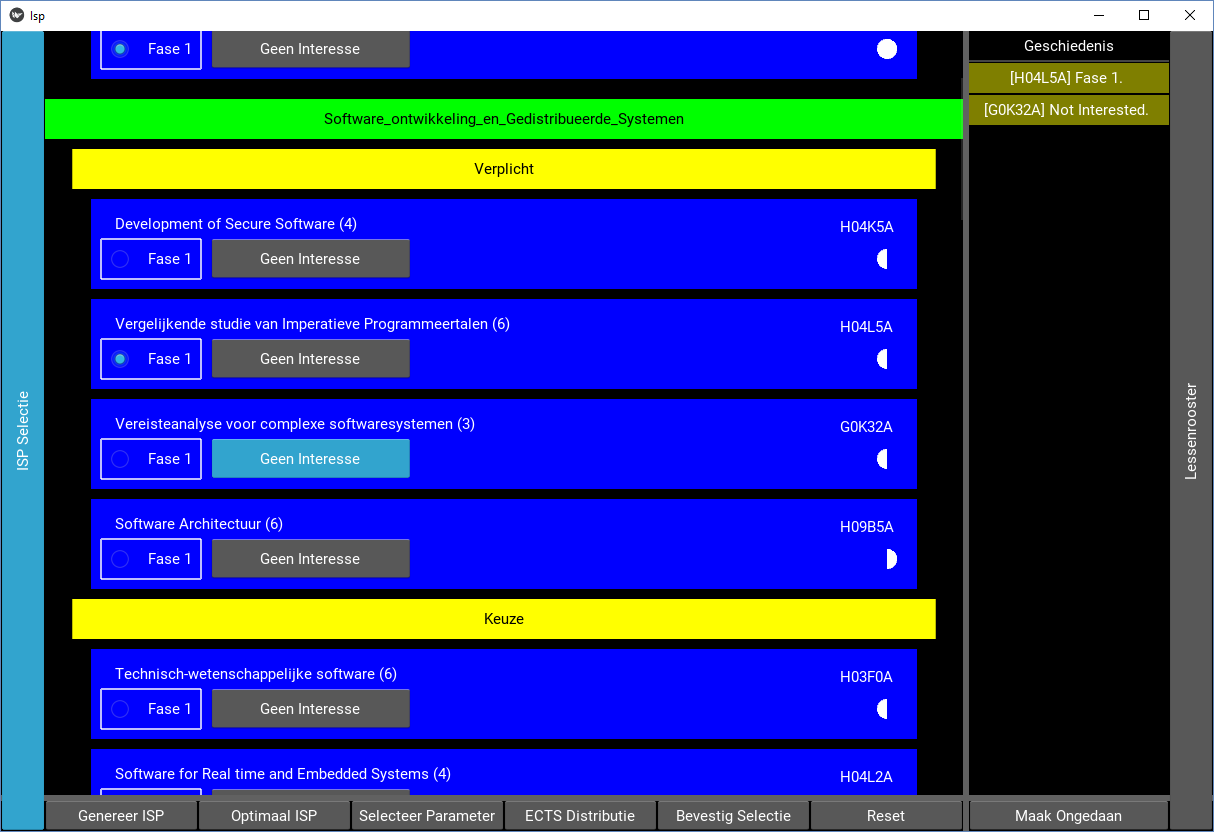
\includegraphics[scale=.35]{sc1.png}
\end{figure}

\paragraph{Overzicht lessenrooster} 
E\'{e}n van de doelstellingen in dit onderzoek is de integratie van het lessenrooster bij het opstellen van het ISP. Het tweede onderdeel van de interface \ref{fig:sc2} is speciaal hiervoor ontworpen. Voor de huidige selectie van de student zal telkens het bijhorende lessenrooster worden bepaald. In dit onderdeel van de applicatie kan de gebruiker een duidelijk overzicht bekijken van dit lessenrooster en eventuele overlap in lesmomenten laten berekenen. Via de kalender kan de student de dagindeling van eender welke werkdag bekijken. Opleidingen bestaan mogelijk uit meerdere fases, linksonder kan de student kiezen voor welke fase van de opleiding hij/zij het lessenrooster wil bekijken. De dagindeling staat weergegeven aan de rechterzijde van het scherm. De knop onderaan rechts berekent de totale overlap van lesmomenten per week.

\begin{figure}
\caption{Het overzicht van het lessenrooster\label{fig:sc2}}
\centering
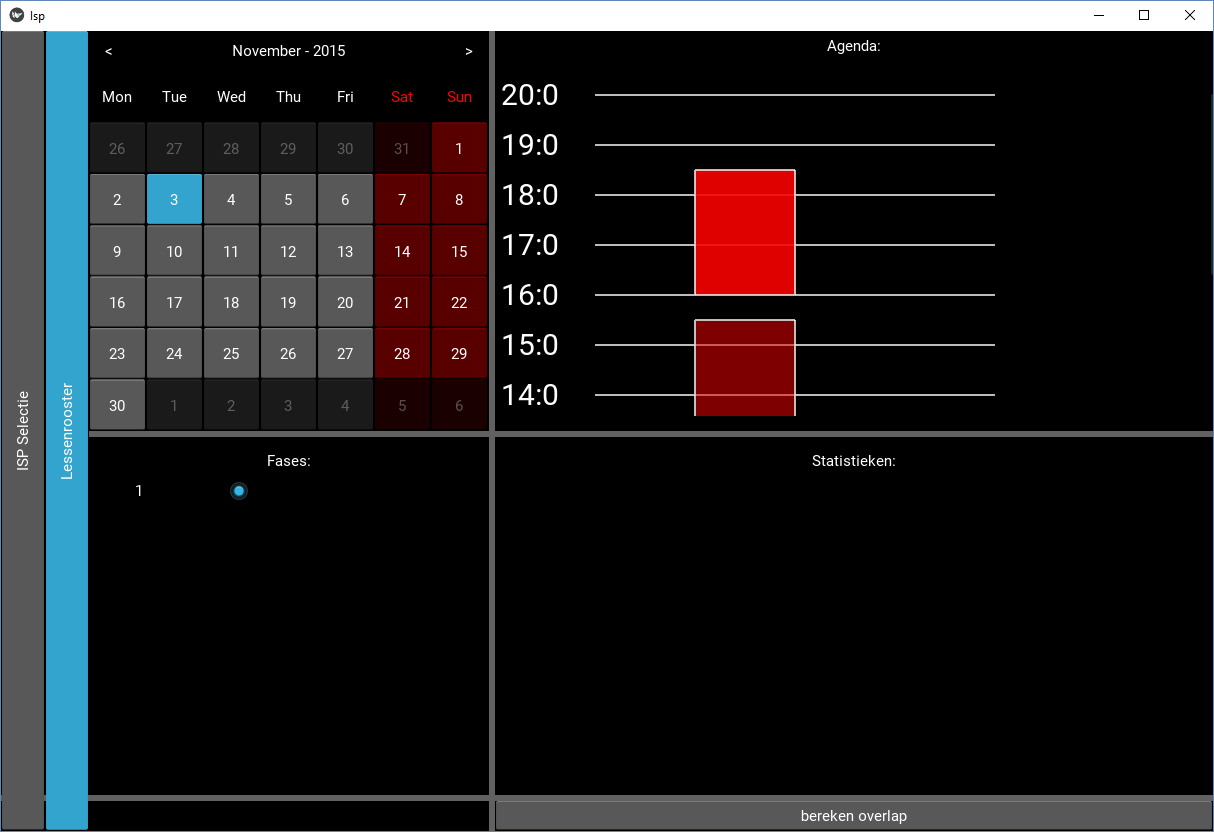
\includegraphics[scale=.35]{sc2.png}
\end{figure}


\subsection{Communicatie tussen Front- en Back-end}
Niet alleen is de syntax tussen IDP en Python compleet verschillend, het zijn ook twee verschillende klassen van programmeertalen respectievelijk declaratief en objectgeori\"{e}nteerd. Dus communicatie tussen de twee talen is niet vanzelfsprekend. Een Python API die toelaat IDP te gebruiken is reeds ontwikkeld \citep{vennekens2015lowering}. Het doel van de API is om de kloof tussen de declaratieve omgeving van IDP en Python kleiner te maken. Door een populaire programmeertaal te kiezen hoopt de auteur dat informatici met een achtergrond in declaratieve talen en logica sneller van IDP gebruik zullen maken zelfs als ze de syntax van IDP niet meester zijn. Persoonlijk heb ik wel al ervaring met IDP en heb dus geopteerd om geen gebruik te maken van de API. De input van IDP is compleet tekstueel, de front-end moet een volledig tekst-bestand genereren in een formaat dat IDP kan begrijpen. De output van IDP is opnieuw een tekst-bestand dat de front-end zal moeten parsen om het resultaat te kunnen verwerken. Zo'n tekst-bestand heeft altijd dezelfde opmaak, het bevat een theorie, vocabularium, structuur, procedure en eventueel termen in geval van minimizatie. De front-end bevat een parser object dat voor elke oproep zo'n tekst bestand zal opbouwen. De theorie, vocabularium en de procedures zijn altijd dezelfde en hoeven slecht \'{e}\'{e}nmalig ingelezen te worden. Enkel de structuur zal bij elke nieuwe actie gedeeltelijk dynamische gegenereerd moeten worden. De interpretatie G voor $\Gamma$ is gegeven, maar de interpretatie W voor $\Omega$ moet bij elke stap opnieuw gegenereerd worden.
\chapter{Evaluatie}
\label{cha:evaluatie}
E\'{e}n de de doelstellingen van dit onderzoek is om na te gaan het mogelijk is een theorie te ontwikkelen in FO(\textperiodcentered) die in staat is alle om alle regels te beschrijven voor een klein domein van opleidingen van de K.U. Leuven. Met deze regels willen we natuurlijk inferentie kunnen doen, en een belangrijke vereiste van een Interactief configuratieprobleem zoals een ISP samenstellen is een snelle respons. De inferentietaken moeten dusdanig snel afgehandeld kunnen worden dat de reactietijd hooguit enkel seconden bedraagt. Deze worden getest d.m.v. een front-end applicatie met een grafische interface die verscheidene functionaliteiten aanbiedt gebaseerd op inferentie taken van het IDP systeem. Hierbij wordt ook het lessenrooster in rekening gebracht, zodat de student een overzicht heeft van het mogelijk lessenrooster dat bij diens keuze van opleidingsonderdelen hoort. En tenslotte is er nog conflict explanation, waarbij ik de mogelijkheden en prestaties van twee methodes wil onderzoeken. De eerste methode is die van reified constraints, die gebaseerd is op technieken die beschikbaar zijn binnen het IDP systeem. De tweede is de compilatie en het gebruik van een eindige toestandsautomaat, die minimale oplossingen voorziet om satisfieerbaarheid te herstellen.

\subsection{Theorie van het ISP}
Geen twee opleidingen zijn dezelfde, en toch zou het gemakkelijk zijn als ongeacht deze verschillen we telkens dezelfde set van regels kunnen gebruiken zonder daarin te moeten gaan aanpassen. Om de omvang van het project haalbaar te houden voor \'{e}\'{e}n persoon, is het domein van opleidingen beperkt gebleven tot die van de computerwetenschappen en toegepaste informatica. Hiervoor ben ik erin geslaagd en theorie op te stellen die zonder probleem eender welk van deze opleidingen kan beschrijven. Hoewel de naamgeving vaak verschilt per opleiding, komen toch vaak structuren voor die dezelfde eigenschappen vertonen. Dus de echte uitdaging is deze structuren vinden, niet de regels ervoor schrijven. Voor een klein sub-domein binnen de opleidingen van de K.U. Leuven is het dus mogelijk een theorie te vinden. 

\subsection{Front-End Applicatie} 
Het hoofddoel van de Front-End (incl. Grafische User Interface) is het simuleren van een mogelijke toekomstige applicatie die effectief gebruikt kan worden door studenten en om gemakkelijk de inferentie technieken van het IDP systeem te kunnen testen in een real-time setting. Momenteel bestaat er al een web applicatie waarmee een student een ISP kan samenstellen. Deze kan als maatstaf dienen in de beoordeling van het nieuwe systeem. Er kan namelijk pas gesproken worden van vooruitgang als de nieuwe toepassing betere prestaties levert en uitgebreidere functionaliteit biedt ten opzichte van de reeds bestaande standaard. Hierbij ligt de focus op (i) het verschil in functionaliteiten (welke functionaliteit is aanwezig in welke applicatie?) en (ii) het niveau van ondersteuning dat ze aanbieden. Criteria zoals design en platform zullen hier niet aan bod komen aangezien deze niet tot de essentie van dit onderzoek behoren. Prestaties van de verschillende inferentie technieken staan besproken in een verder hoofdstuk. 

De huidige web applicatie van de K.U. Leuven biedt een basispakket van ondersteuning aan, essentieel voor de student om zijn/haar ISP te kunnen vervolledigen. Het laat de student toe om te kiezen welke opleidingsonderdelen van de gekozen opleiding hij/zij van plan is te volgen. De selectie kan vervolgens gecontroleerd worden op correctie, m.a.w. het systeem zal nagaan of ze voldoet aan alle regels van het ISP. En als de selectie niet voldoet aan deze regels zal het systeem dit melden en tevens ook uitleg voorzien waarom de selectie niet voldoet aan de regels. Deze functionaliteiten zitten ook allemaal inbegrepen in de nieuwe applicatie, samen met nog een aantal nieuwe functies. Hiermee kan ik veilig stellen dat het aanbod van functionaliteit in mijn nieuwe applicatie zeker uitgebreider is dan dat van het huidige systeem. 
Naast het basispakket is het ook mogelijk voor de gebruiker om een parti\"{e}le selectie verder te laten invullen door het systeem tot het een volledig geldige selectie is volgens de regels van het ISP, het is zelfs mogelijk om een optimaal ISP te laten opstellen volgens een bepaald criterium. Gedurende het selectieproces is het mogelijk dat de keuzes van gebruiker ervoor zorgen dat bepaalde opleidingsonderdelen geselecteerd moeten worden als een gevolg hiervan, het systeem zal deze keuzes automatisch invullen (propageren) zodat de gebruiker zich hier geen zorgen over moet maken. Elke nieuwe stap in het selectieproces wordt bijgehouden in een geschiedenis van acties, als de gebruiker niet tevreden is met de selectie en deze wil wissen dan kan dit door de acties ongedaan te maken. Wanneer de student een vak selecteert dan zal het systeem een partieel lessenrooster genereren, dit is handig om te controleren of mogelijk geen lesmomenten overlappen met elkaar. 

\begin{table}[]
\centering
\caption{Functionaliteiten}
\label{functionaliteiten}
\begin{tabular}{|l|c|c|}
\hline
 & Web applicatie & Nieuwe applicatie \\ \hline
Handmatige selectie & \checkmark & \checkmark \\ \hline
Controle correctheid & \checkmark & \checkmark \\ \hline
Verklaring v. incorrectheid & \checkmark & \checkmark \\ \hline
ISP genereren &  & \checkmark \\ \hline
Optimaal ISP genereren &  & \checkmark \\ \hline
Propagatie &  & \checkmark \\ \hline
Ongedaan maken & \checkmark & \checkmark \\ \hline
Geschiedenis v. Acties &  & \checkmark \\ \hline
Weergave lessenrooster &  & \checkmark \\ \hline
\end{tabular}
\end{table}

Er is dus een duidelijk verschil in het aanbod van functionaliteiten, maar de voordelen van deze nieuwe mogelijkheden mogen niet te koste gaan van het niveau van ondersteuning dat de functionaliteiten van het bestaande systeem bieden. Elke functionaliteit van het nieuwe systeem wordt beschreven en eventueel vergeleken met de gelijkaardige functionaliteit uit de web applicatie van het K.U. Loket. 

Als eerste is er de handmatige selectie, wellicht de meest essenti\"{e}le van alle functionaliteiten. In beide applicaties geeft het de student de mogelijkheid om aan te vinken welke van de vakken hij/zij wenst te volgen, beide applicaties werken op dezelfde manier met uitzondering dat het in de web applicatie niet mogelijk is om aan te geven dat je niet ge\"{i}nteresseerd bent in een vak. 

Zowel de bestaande als de nieuwe app kunnen een selectie controleren op geldigheid, maar de nieuwe applicatie doet dit bij elke nieuwe selectie van de student zodanig dat fouten zo snel mogelijk gedetecteerd worden. Bij de web applicatie gebeurt dit enkel wanneer de student denkt klaar te zijn en diens keuze bevestigt. 

Blijkt dan dat de selectie niet geldig is volgens de regels, dan dient hier een verklaring voor gegeven te worden. Het bestaande systeem biedt duidelijke verklaringen in de zin dat het kan verklaren welke regels er niet kloppen. De duidelijkheid van de verklaringen in het nieuwe systeem is sterk afhankelijk van de IDP theorie die het gebruikt, de opmerking werd al gemaakt dat een algemene theorie niet geschikt is om de gebruiker goed te kunnen informeren i.p.v. een specifieke theorie. Het is dus mogelijk voor de nieuwe applicatie om evenveel duidelijkheid te kunnen scheppen als de web applicatie, maar dit zal sterk afhangen van de gebruikte theorie en dus ten koste zijn van andere factoren. Maar hier houdt het voor de web applicatie op, naast tekstuele verklaringen van de regels die verbroken zijn biedt het systeem geen verdere ondersteuning die de gebruiker kunnen helpen bij het oplossen van een foute selectie. De nieuwe applicatie kan opsporen in welk deel van de selectie de fout zich bevindt, en is zelfs in staat om alle mogelijk (minimale) oplossingen te tonen aan de gebruiker. 

Het bijhouden van de acties gemaakt door de gebruiker in een geschiedenis is ook \'{e}\'{e}n van de nieuwe features. Voorheen was het al mogelijk om selecties ongedaan te maken door simpelweg het vinkje in de checkbox van een geselecteerd vak uit te vinken. Dit is nog altijd mogelijk maar daarbij is het ook nog eens mogelijk om de acties uit de geschiedenis ongedaan te maken. Propagaties die niet meer gelden als gevolg van acties of selecties ongedaan maken zullen getoond worden aan de student die dan kan kiezen of hij/zij deze nog wil behouden of niet. 

En tenslotte kan de student een parti\"{e}le selectie verder laten vervolledigen door het systeem. Hierbij zal het systeem uiteraard de reeds gemaakte keuzes behouden en ze verder vervolledigen. De student kan aangeven als hij/zij niet ge\"{i}nteresseerd is in bepaalde vakken en bij het verder aanvullen van de selectie zal de nieuwe applicatie deze vakken niet kiezen. Niet alleen is het mogelijk om een parti\"{e}le selectie verder aan te vullen, maar de student kan als hij/zij dit wenst een optimaal ISP samen laten stellen volgens een bepaalde parameter (bv. de werklast zo gelijk mogelijk verdelen over beide semesters). 

\subsection{Inferentie} 
Met behulp van de interface kan de gebruiker een ISP samenstellen. Het is de bedoeling om de gebruiker bij te staan in dit proces, dit door gevolgen van bepaalde keuzes door te voeren, een onvolledige selectie te vervolledigen, een optimaal ISP samen te stellen volgens een bepaald criterium, foute keuzes te detecteren en de gebruiker hiervan op de hoogte te brengen etc.. En niet te vergeten, al deze processen moeten in real-time gebeuren en dus zeer snel afgehandeld kunnen worden. Binnen het domein van de opleidingen, ben ik tot de conclusie gekomen dat zowat al deze inferentie taken snel zeer snel en effici\"{e}nt uitgevoerd worden. De reactietijd, meegerekend het genereren van de IDP text file en het resultaat terug ontcijferen bedraagt in bijna alle gevallen minder dan 1 seconde. Zelfs de resultaten van minimizatie opdrachten geven goede resultaten terug met een maximale rekentijd van ongeveer 10 seconden. 

/*RESULTATEN*/

\subsection{Conflict Explanation} 
Voor IC problemen is het de verantwoordelijkheid van het systeem om de gebruiker zo goed mogelijk bij te staan terwijl deze het probleem probeert op te lossen. Dit geldt zeker voor situaties waarbij de gebruiker een keuze heeft gemaakt die nooit tot een geldige oplossing kan leiden. In dit onderzoek heb ik de prestaties van twee technieken onderzocht, als eerste is er de techniek van reified constraints die enkel gebruik maakt van de inferentie taken binnen het IDP systeem. De tweede techniek is een combinatie van IDP met die van Amilhastre.

\subsubsection{Reified Constraints}
De techniek van reified constraints biedt extra informatie en kan dienen als een helpende hand om de gebruiker door het selectieproces te loodsen. Deze simpele generische manier om niet-satisfieerbare regels op te sporen en te verklaren in natuurlijke taal heeft zeker zijn voordelen. De implementatiekost ligt zeer laag, maar de functionaliteit van deze techniek is helaas ook beperkt. Door de techniek te combineren met de unsatstructure is het mogelijk om niet-satisfieerbare regels effici\"{e}nt op te sporen. En door aan elke regel een uitleg in natuurlijk taal te koppelen (deze hoeft slechts \'{e}\'{e}nmalig per regel opgesteld te worden) kan het systeem de gebruiker een beter begrijpbare ondersteuning bieden door precies te zeggen welke regel(s) er verbroken is (zijn) en te specifi\"{e}ren hoe dit zou kunnen gebeurd zijn. Maar deze uitleg is zeer statisch, dus als dezelfde regel door verschillende keuzes verbroken wordt zal de uitleg in beide gevallen dezelfde zijn. In vele gevallen is deze informatie duidelijk en specifiek genoeg, maar in de implementatie staat ook een voorbeeld vermeld waarbij de uitleg niet veel extra hulp biedt omdat de regel die ze beschrijft te algemeen is. Sinds het de bedoeling is van dit onderzoek om een zo algemeen mogelijke theorie te ontwikkelen kan de vraag gesteld worden hoe nuttig het is om deze techniek te gebruiken in combinatie met dit concept. Momenteel is de scope van opleidingen nog z\'{e}\'{e}r beperkt en zelfs dan bestaan er al regels die te algemeen zijn een duidelijk beeld te kunnen scheppen van wat er precies mis zou kunnen zijn. In een poging om de theorie nog algemener te maken zodat nog meer opleidingen beschreven kunnen worden, bleken de regels zo algemeen te worden dat een beschrijving in natuurlijke taal niet langer nuttig was. Dus waarschijnlijk zal er een afweging moeten gemaakt worden tussen een algemene theorie die zoveel mogelijk opleidingen kan beschrijven of duidelijke uitleg kunnen bieden ten koste van de uitdrukkingskracht van de theorie.

\subsubsection{Eindige toestandsautomaat}
\paragraph{Constructie}
Een tweede vorm van conflict explanation in dit werk is het voorzien van oplossingen, oftewel precisie minimale subsets die ongedaan dienen gemaakt te worden om satisfieerbaarheid te herstellen. Om dit te bereiken heb ik mij gebaseerd op het werk van \citep{amilhastre2002consistency}. Het gebruik van de automaat laat toe om deze oplossingen te berkerenen. Deze automaat moet op voorhand \'{e}\'{e}nmaal berekend worden, waarna ze bewaard wordt om eender wanneer te kunnen gebruiken. Het is mogelijk om de automaat te construeren met behulp van model expansie, waarbij IDP alle modellen berekent en opsomt. De bouw van de automaat gebeurt in verschillende stappen. 
\begin{enumerate}
\item Alle modellen worden opgesomd d.m.v. model expansie in IDP
\item De modellen worden vertaald naar een formaat dat nodig is om een automaat mee te bouwen.
\item Een automaat wordt gebouwd \ref{alg:fsaConstructie}.
\item De automaat wordt herleid tot een minimale automaat m.b.v. het algoritme van Hopcroft.
\end{enumerate}
In de tabel \ref{tab:compilatie} staan de resultaten van de bouw van twee automaten voor de opleidingen master toegepaste informatica en master computerwetenschappen. De tijd die nodig is voor de constructie is redelijk gezien zo op voorhand gebeurt en slechts \'{e}\'{e}nmaal uitgevoerd moet worden.
\begin{table}[]
\centering
\caption{Resultaten compilatie}
\label{tab:compilatie}
\begin{tabular}{|l|l|l|}
\hline
 & Toegepaste Informatica & Computerwetenschappen \\ \hline
1 &  &  \\ \hline
2 &  &  \\ \hline
3 &  &  \\ \hline
4 &  &  \\ \hline
Totaal: &  &  \\ \hline
\end{tabular}
\end{table}

\paragraph{Gebruik}
Gebruik makend van deze automaat worden de oplossingen berekend,  het berekenen van deze oplossingen kan gedaan worden in tijd polynomiaal met betrekking tot de grootte van het resultaat. De prestaties van deze techniek voor het ISP probleem zijn te zien in /*REF TABLE*/. Naast het berekenen van oplossingen zijn er nog andere inferentie technieken mogelijk op basis van de automaat, maar deze worden niet toegepast in dit onderzoek.

\subsection{Evaluatie van het Configuratiesysteem}
In de introductie werd er verwezen naar het werk van \citep{van2016kb}, en meer specifiek naar de gebruikte evaluatiemethode. IDP werd ge\"{e}valueerd volgens negen criteria uit \citep{felfernig2014knowledge} die bedoeld zijn om een beter beeld te geven van de prestaties van configuratiesystemen. IDP bleek te voldoen aan de meeste van criteria, en in een vergelijking met tien andere bekende configuratiesystemen kwam IDP als een van de sterkste systeem uit de bus. 

Nemen we even terug criterium (C3) \textit{Automated Consistency Maintenance}, oftewel de aanwezigheid van een manier om consistentie te onderhouden tijdens het ontwikkelen van de theorie (a priori) zowel als gedurende het selectieproces (runtime). Het IDP systeem heeft hier slechts parti\"{e}le ondersteuning voor. A priori is automated consistency maintenancy volledig ondersteund, en in theorie ook gedurende het selectieproces. Maar door computationele beperkingen is dit sterk afhankelijk van de omvang van het probleem. Als alternatief kan er beroep gedaan worden op benaderingen, maar die hebben helaas niet dezelfde garanties. 

De methode volgens Amilhastre heeft een aantal garanties, waaronder ook consistency maintenance. De kost van een selecties toevoegen of ongedaan maken is lineair met betrekking tot de grootte van de automaat. Hoewel deze grootte in het slechtste geval exponentieel is, is de grootte in de praktijk echter redelijk. Dit heeft twee redenen, in geval van IC problemen zijn veel van de domeinwaarden onderling verwisselbaar en is de structuur van een probleem opgedeeld in subproblemen die min of meer onafhankelijk zijn van elkaar. De garantie van deze eigenschap is belangrijk, omdat het toevoegen van selecties en het verwijderen ervan rechtstreeks in verband staat met consistency maintenance. Door het toevoegen of verwijderen van selecties worden de kosten van de paden in de automaat aangepast (in tijd lineair m.b.t. de grootte ervan). Controleren of een selectie satisfieerbaar is (in deze context consistency maintenance genoemd) wordt gedaan op basis van deze kost en heeft een complexiteit van \textit{O(1)}. De combinatie van de twee zorgt er dus voor dat voldaan wordt aan voorwaarde C3. 

\begin{table}[]
\centering
\caption{IDP vs IDP+FSA}
\label{criteria}
\begin{tabular}{|l|c|c|}
\hline
 & IDP & IDP + FSA \\ \hline
C1 & - & - \\ \hline
C2 & $\checkmark$ & $\checkmark$ \\ \hline
C3 & $\approx$ & $\checkmark$ \\ \hline
C4 & $\checkmark$ & $\checkmark$ \\ \hline
C5 & $\checkmark$ & $\checkmark$ \\ \hline
C6 & $\checkmark$ & $\checkmark$ \\ \hline
C7 & $\approx$ & $\approx$ \\ \hline
C8 & $\checkmark$ & $\checkmark$ \\ \hline
C9 & $\checkmark$ & $\checkmark$ \\ \hline
\end{tabular}
\end{table}
\chapter{Besluit}
\label{cha:besluit}
\paragraph{Proof of concept}
De eerste onderzoeksvraag die gesteld werd in dit onderzoek was de vraag of het mogelijk was om met behulp van IDP een theorie te ontwikkelen voor het ISP probleem en belangrijker nog of we effici\"{e}nt inferentie kunnen doen met deze theorie. De voordelen van de uitdrukkingskracht van FO(\textperiodcentered) zijn al vaker aangehaald \cite{van2016kb} \cite{de2014predicate} in het verleden. En voor het huidige probleem houden deze beweringen opnieuw stand, sinds ik met behulp van FO(\textperiodcentered) erin geslaagd ben om een theorie te ontwikkelen die in staat is om voor een klein domein binnen de opleidingen aan de universiteit de geldige samenstellingen voor het ISP te beschrijven.
In IDP en het concept van kennisbank-systemen is er een strikte scheiding tussen kennis en inferentie. De theorie wordt slechts \'{e}\'{e}nmaal beschreven en deze laten toe om meerdere vragen te beantwoorden d.m.v. verschillende vormen van inferentie toe te passen op de theorie. Dit is enkel nuttig als deze inferentie technieken effici\"{e}nt en snel genoeg werken om ze in een interactieve context te kunnen gebruiken. Het testen van deze technieken werd gedaan met behulp van de zelf ontwikkelde front-end applicatie. Voor alle gebruikte technieken bleken de reactiesnelheden te voldoen aan de vereisten van een interactief configuratieprobleem. Zelfs voor de meest complexe bewerkingen (bv. minimizatie) boekt het IDP systeem goede resultaten. Dus met dit proof of concept wordt opnieuw de kracht van FO(\textperiodcentered) getoond samen met de prestaties van de inferentie methoden binnen het het kennisbank paradigma.

\paragraph{Conflict explanation}
Meerdere onderzoeken hebben de voordelen van declaratieve methoden \cite{gelle1996interactive} en specifiek die van KB-systemen \cite{de2014predicate} \cite{denecker2008building} \cite{van2016kb} \cite{vlaeminck2009logical} ten opzichte van imperatieve strategie\"{e}n al aangehaald. Dit betekent niet dat een declaratieve aanpak op alle vlakken beter is, en of dat alle vragen rond declaratieve systemen beantwoord zijn. Binnen het domein van conflict explanation zijn er reeds verschillende technieken ontworpen voor het zoeken naar, verklaren en oplossen van conflict situaties binnen IC problemen. Elke techniek hangt samen met zijn eigen concept van wat een oplossing juist is en hoe deze geformuleerd hoort te worden. In deze paper heb ik een aantal interessante technieken ge\"{i}mplementeerd en de resultaten ervan beschreven. De eerste, reified constraints maken enkel gebruik van de tools beschikbaar in IDP terwijl de tweede methode technieken combineert binnen IDP met die uit het werk van \citep{amilhastre2002consistency}. Reified constraints is een techniek met lage implementatiekost waarmee verklaringen in natuurlijke taal kunnen gegeven worden voor regels die verbroken zijn. De duidelijkheid van de verklaringen blijkt sterk af te hangen van de theorie, en daarbij is de uitleg zeer statisch. Afhankelijk van het probleem kan overwogen worden om gebruik te maken van reified constraint. De laatste techniek tenslotte, gebruikt een automaat voor het berekenen van minimale oplossingen om de selectie terug satisfieerbaar te maken. De manier waarop deze automaat wordt gebouwd is z\'{e}\'{e}r interessant omdat het gebruik maakt van model expansie, een inferentie techniek die ingebouwd zit in IDP. De resultaten van deze automaat zijn heel positief en het feit dat ze kan gebouwd worden met behulp van IDP biedt mogelijkheden voor de toekomst. 


\chapter{Toekomstig Werk}
\label{cha:toekomstigwerk}
Voor een klein domein van opleidingen is het gelukt om een theorie te ontwerpen met behulp van FO(\textperiodcentered). Natuurlijk is het aantal opleidingen binnen de K.U. Leuven aanzienlijk groter. Dus achterhalen of het mogelijk is om een theorie te ontwikkelen die om kan gaan met alle opleidingen, is werk voor de toekomst. Maar ik zou niet enkel zoeken naar aan antwoord op dit probleem maar ook naar alternatieven zoeken, bijvoorbeeld \'{e}\'{e}n theorie per type opleiding. Bachelor opleidingen hebben vaak meer gemeen met andere bachelor opleidingen, dan met bijvoorbeeld master studies. Het zou zeker interessant zijn om te kijken wat de mogelijkheden hieromtrent zijn en voor- en nadelen die hiermee gepaard gaan. 

De prestaties van de inferentie technieken van IDP voor het ISP probleem zijn positief en voldoen aan de vereisten van een IC probleem. De front-end is in staat om alle functionaliteit van de bestaande web applicatie aan te bieden met toevoeging van nieuwe functionaliteiten. Deze steunen \textit{bijna} allemaal op de technieken die in IDP te vinden zijn. Deze succesvolle steekproef op een klein subdomein van opleidingen leidt mij tot de conclusie dat er meer mogelijk is. Hopelijk zijn deze resultaten een motivatie voor anderen om verder uit te zoeken wat de mogelijkheden zijn van IDP met betrekkingen tot het ISP probleem en andere (als niet alle) opleidingen aan de K.U. Leuven en misschien zelfs andere onderwijsinstellingen. 

Door gebruik te maken van de automaat die beschreven staat in het werk van Amilhastre et al. is het gelukt om minimale correcties te kunnen berekenen. Opvallend hierbij is dat de bouw hiervan kan gebeuren op basis van model expansie in IDP. Het onderzoek rond IDP is nog altijd volop bezig, en een nieuwe versie van het systeem wordt momenteel ontwikkeld. Gezien de voordelen van het gebruik van zo'n automaat zou het zeer interessant zijn om te zien of het werk van Amilhastre niet ge\"{i}ntegreerd kan worden in een toekomstige versie van het systeem. Het werk van \citet{fargier2004compiling} is een uitbreiding op dat van Amilhastre en Vempaty. Fargier stelt het gebruik van Tree-driven automata voor, een nog compactere weergave waarbij de positieve eigenschappen van voorheen blijven gelden. En verder onderzoek zal antwoordt moeten bieden of deze techniek eventueel ook gecombineerd zou kunnen worden met het IDP systeem.

\backmatter
% Na de bijlagen plaatst men nog de bibliografie.
% Je kan de  standaard "abbrv" bibliografiestijl vervangen door een andere.
\bibliographystyle{abbrv}
\bibliography{referenties}

\end{document}

%%% Local Variables: 
%%% mode: latex
%%% TeX-master: t
%%% End: 
